\documentclass{article}

\usepackage{corl_2020} % Use this for the initial submission.
%\usepackage[final]{corl_2020} % Uncomment for the camera-ready ``final'' version.

\usepackage{graphicx}
\usepackage{url}
\usepackage{amsmath}
\usepackage{amsfonts}
\usepackage{mathtools}
\usepackage{caption}
\usepackage{subcaption}
%\usepackage{xcolor}
\usepackage{wrapfig}
\usepackage{float}

\title{End-to-end learned autonomous off-road navigation using a physics-based simulation framework}

% Reinforcement learning using end-to-end networks for off-road autonomous navigation

% Reinforcement learned for off-road autonomous navigation using physics-based simulation

% The \author macro works with any number of authors. There are two
% commands used to separate the names and addresses of multiple
% authors: \And and \AND.
%
% Using \And between authors leaves it to LaTeX to determine where to
% break the lines. Using \AND forces a line break at that point. So,
% if LaTeX puts 3 of 4 authors names on the first line, and the last
% on the second line, try using \AND instead of \And before the third
% author name.

% NOTE: authors will be visible only in the camera-ready (ie, when using the option 'final'). 
% 	For the initial submission the authors will be anonymized.

\author{
  Asher Elmquist \\
  Department of Mechanical Engineering \\
  University of Wisconsin-Madison \\
  Madison WI, USA \\
  amelmquist@wisc.edu \\
  \And
  Simone Benatti \\
  Dipartimento di Ingegneria ed Architettura \\
  Università di Parma \\
  Parma, Italy \\
  simone.benatti@studenti.unipr.it \\
  \And
  Aaron Young \\
  Department of Mechanical Engineering \\
  University of Wisconsin-Madison \\
  Madison WI, USA \\
  aryoung5@wisc.edu \\
  \And
  Alessandro Tasora \\
  Dipartimento di Ingegneria ed Architettura \\
  Università di Parma \\
  Parma, Italy \\
  alessandro.tasora@unipr.it \\
  \And
  Radu Serban \\
  Department of Mechanical Engineering \\
  University of Wisconsin-Madison \\
  Madison WI, USA \\
  serban@wisc.edu \\
  \And
  Dan Negrut  \\
  Department of Mechanical Engineering \\
  University of Wisconsin-Madison \\
  Madison WI, USA \\
  negrut@wisc.edu \\
}


\newcommand{\todo}[1]{\textcolor{red}{\textbf{#1}}}

% highlighting, coloring, etc.
\newcommand{\highlightThis}[1]{\textcolor{red}{{\bf{{#1}}}}}
\newcommand{\highlight}[1]{\textcolor{red}{#1}}
\newcommand{\textcolorRED}[1]{{\textcolor{red}{#1}}}
\newcommand{\textcolorBLACK}[1]{{\textcolor{black}{#1}}}


\newcommand{\softpackage}[1]{{\sffamily{#1}}}
\newcommand{\CHRONO}{{\softpackage{{Chrono}}}}

\newcommand{\sbelNewSolution}[1]{\medskip\noindent{\textit{#1}}}


\begin{document}
\maketitle

%===============================================================================

\begin{abstract}
This contribution discusses an end-to-end reinforcement learning approach for off-road autonomous vehicle (AV) navigation. Both learning and testing are done in simulation. The contribution highlights: ($i$) the strategy employed for end-to-end learning; and ($ii$) the simulation infrastructure used to learn and test the control policy. For ($i$), we use sensor data fusion (camera, GPS, and IMU). For ($ii$), we developed a physics-based, open source integrated simulation environment that supports vehicle dynamics, deformable/undeformable terrains, and virtual sensing. We use a Gator off-road vehicle to demonstrate how a policy learned on flat undeformable terrain performs when used in hilly conditions while navigating around a course of randomly placed obstacles. The hilly terrain covers a swath of 80$ \times $80 meters and the soil can everywhere be either undeformable, or deformable hard (silt-like), or deformable soft (snow-like). The results reported herein can be reproduced with models and data available in a public repository \cite{CoRLsupportData2020}. Movies associated with the tests run are available online  \cite{CoRLpaperVideos2020}.
%The policy is learned on rigid-terrain, with uneven terrain before being deployed in an environment with deformable terrain, and additional terrain obstacles to test and understand robustness. This study flexes an open-source software platform that supports robot and autonomous vehicle simulation by providing support for vehicle dynamics, deformable terrain, and virtual sensors. The learned policy is tested for robustness in the environment to understand the policy's ability to successfully and consistently navigate a complex off-road environment and test the sensitivity of the policy to the training environment. 

\end{abstract}

% Two or three meaningful keywords should be added here
\keywords{Simulation, Reinforcement Learning, Off-road Autonomous Vehicles, Deformable Terrain} 

%===============================================================================

%!TEX root = ../main.tex



\section{Introduction}

We use physics-based simulation to produce end-to-end policies for controlling AV navigation directly from raw sensory data. The AVs operate in hilly, off-road conditions with randomly placed obstacles (rocks) obstructing safe navigation. Training is based on a curriculum learning approach; the complexity of the environment is increased as the policy converges. The training is exclusively done with undeformable terrain since these simulations run faster than real time \cite{negrutGVSETS2020}. In the current implementation, deformable terrain simulation is approximately 100$ \times $ slower than the undeformable counterpart. As such, learning on deformable terrain is expensive. The control policy derived is tested on deformable soils that have different textures and soil deformation attributes. The deformable soils are of two categories: deformable but hard (silt-like), and deformable but soft (snow-like). The end-to-end approach to navigation is certainly not new, see, for instance \cite{end2endNVIDIA2016,AminiRKR19}. However, to the best of our knowledge, ($a$) this is the first example of off-road navigation (driving control + reaching a goal) with reinforcement learning; and, ($b$) the simulation environment developed is the first \textit{open-source}, physics-based platform that brings together tracked/wheeled vehicle dynamics, sensor, and terrain simulation. %While the authors acknowledge that it is commonly known that simulated sensor data, specifically rendered camera images, do not directly translate well to reality, other contributions have focused on methods for bridging this gap, and this is not the focus of this paper.

Our goal is to demonstrate that off-road mobility of AVs can rely on simulation for the development of control policies; and, to report on tests that assess these policies' effectiveness. We do not comment on the transferability of the derived control policies \cite{sim2realGapEssex1995}. Rather than addressing this important issue, for which we actually do not have an answer yet, this contribution focuses on the learning and the platform that enabled it, including probing the robustness of the policy in simulation. Thus, in \S\ref{sec:relatedWork} we provide an overview of similar ongoing efforts in the simulation-in-robotics area. Section \S\ref{sec:simEnv} provides an outline of the simulation environment developed by this group. Section \S\ref{sec:end2endLearning} presents the end-to-end learning approached for off-road AV mobility. Simulation results are described in \S\ref{sec:demoTechnology}. The last section contains concluding remarks and directions of future work.


%!TEX root = ../main.tex

\section{Related Work}
\label{sec:relatedWork}

%This section provides a summary of the state of the art in four areas: simulation engines (\S\ref{subsec:dynamicsEngines}); sensing simulation (\S\ref{subsec:sensingSimulation}); techniques used for learning (\S\ref{subsec:learningTechniques}); and software environments for learning automation (\S\ref{subsec:learningTechniques}).

This section provides a summary of the state of the art in simulation environments (\S\ref{subsec:simEnvironments}), and learning techniques for autonomous navigation (\S\ref{subsec:learningTechniques}). The discussion of simulation environments is restricted to those commonly used for training reinforcement learning algorithms.

\subsection{Simulation Environments for Reinforcement Learning}
\label{subsec:simEnvironments}

Gazebo \cite{koenig2004design}, one of the most broadly used simulators in robotics, has been used for reinforcement learning by leveraging the open-source nature and tight integration with ROS. Gazebo exposes an environment that wraps multiple dynamics engines and sensors. However, it lacks specific support for vehicle modeling and deformable terrain for off-road scenarios.

Widely used for ``in-door robotics'' reinforcement learning, MuJoCo \cite{todorovMujoco2012} is a dynamics engine that supports URDF-based modeling. MuJoCo is not open-source and it does not support high-fidelity vehicle dynamics with deformable terrain interaction which can dominate many off-road maneuvers. The sensing support is also limited due to the simplicity of the noise models that can be applied to the sensors, most of which are restricted to dynamics-based interoceptive sensors. 

An open-source alternative to MuJoCo is PyBullet \cite{matas2018simtoreal}, which exposes many of the same features but also lacks sophisticated sensing support. PyBullet provides an interface to generate the specific sensor data desired by the user. The strengths of PyBullet are in rigid-body dynamics and ease of use, making it a convenient choice for simpler RL applications, but limiting for off-road navigation.

In a more vehicle-centric approach, CARLA \cite{carlaAVsim2017}, AirSim \cite{shah2018airsim}, and Torcs \cite{torcsRacingSimulation2020} all seek to allow vehicle simulation for training and testing of control algorithms. While these are vehicle-focused, they cannot perform off-road simulation and have limited sensor fidelity. Torcs, which is originally based on a racing game, provides limited support for sensing, allowing access to camera and simplified lidar, with dynamic information available directly from the physics engine. CARLA and AirSim are designed for on-road applications and support an array of sensors. The sensors include basic distortions and noise. Due to limited geometric fidelity and time-resolution of collision-based ray-casting, the sensor data is typically overly clean or has obvious discontinuities or modeling artifacts. None of these on-road simulation environments support complex off-road navigation.


%%%%%%%%%%%%%%%%%%%%%%%%%% SIMONE
\subsection{Learning techniques}
\label{subsec:learningTechniques}

Deep Reinforcement Learning (DRL) techniques have shown outstanding level of performance since their very introduction \cite{Mnih13}. Subsequently, DRL has been used in vision-based robotic manipulation tasks. Robots controlled by DRL-trained neural networks (NN) have been shown to solve complex tasks in unstructured environments with \cite{zhu2018reinforcement} or without \cite{LevineFDA15} the use of imitation learning. 
End-to-end RL approaches have also been successfully applied to on-road autonomous driving. One of the major challenges in this area is the gap between RGB images generated by simulators and real world camera images, that can cause the autonomous driving policies trained in simulation to perform poorly in the real world. This issues has been addressed in various ways, such as using synthesized realistic images \cite{YurongALDriving17} or tools to generate images directly from real-world sampling \cite{Amini2020RLDriving}.

Sensor fusion with DRL techniques have shown promising results in controlling small indoor robots with camera + LiDAR \cite{BohezVCVSD17,PatelCKK2017}. RL in conjunction with imitation learning have been used for off-road driving when the vehicle learned to run laps quickly  \cite{Pan2017OffRoadAV}. However, to the best of our knowledge, there has been no demonstration of an end-to-end, off-road driving policy capable of reaching a target position while avoiding randomly placed obstacles on deformable soil and hilly terrain. 

%!TEX root = ../main.tex

\section{Chrono Simulation Environment}
\label{sec:simEnv}
The physics-based simulator used in conjunction with this work is called Chrono. It is actively developed, it is open source, and it is released under a permissive BSD3 license for unfettered use/change/distribution \cite{projectChronoGithub}. A full description of the simulation platform falls outside the scope of this document; for an overview, see \cite{chronoOverview2016}. Chrono provides support for multibody dynamics (multi-core), nonlinear finite element analysis (multi-core), fluid solid interaction (GPU), granular dynamics (GPU), terramechanics (multi-core/GPU/MPI), sensing (GPU), and the simulation of large collections of AVs running in one joint scenario (MPI). The hardware support is as follows: multi-core CPUs, GPU computing via CUDA, and distributed memory (clusters/supercomputers) via the Message Passing Interface (MPI) standard. The four Chrono components relevant herein are: Chrono::Engine, Chrono::Vehicle, terramechanics, and Chrono::Sensor. Chrono::Engine is the solver that advances the simulation in time. Chrono::Vehicle provides support for rapidly setting up and analyzing vehicles (tracked or wheeled) via a library of templates for vehicle components (suspensions, steering systems, tires, powertrains/diverlines, tracks, etc.) \cite{ChronoVehicle2019}. The terramechanics support comes in three flavors: expeditious and semi-empirical approaches \cite{alessandroSCM2019}, via continuum representations, and using the discrete element method (fully resolved granular terrain).

Sensing support in Chrono is provided as an additional module that sits on top of Chrono::Engine to provide measurement data from inside the simulation and virtual environment. Currently, there is support for RGB cameras, lidar, GPS, and IMU \cite{TR-2020-07}. The sensor module's purpose is to provide realistic data for training and testing autonomous controls. For GPS and IMU, ground truth data, queried from Chrono::Engine is augmented to introduce noise commonly found on accelerometers and gyroscopes \cite{shah2018airsim} as well as GPS receivers. For camera and lidar, the visual environment is ray traced using custom GPU kernels that model the acquisition process of the specific sensor. The ray-traced data is then augmented to introduce noise and distortion to model the true sensor output. All sensors are parameterized by their update frequencies, noise characteristics, and lag. 

Our lidar model augments ground-truth data with noise (based on the measurements of range, intensity, and angular precision) to produce the final point cloud. The lidar leverages ray-tracing to create a point cloud based on the visual scene. This, in combination with supersampling for beam divergence, allows Chrono::Sensor to generate high-fidelity point clouds of complex environments. The beam discretization model extends that proposed in \cite{goodin2018enabling} to allow a user-defined number of rays per lidar beam. By incorporating beam divergence, we can model multiple return modes and encountered objects. In addition to beam divergence, the ray-tracing method allows the temporal sampling of a scanning lidar to be based on modern motion blurring techniques resulting in realistic and continuous distortions that are not possible with large time steps in video gaming collision detection systems employed by other learning environments, e.g. \cite{shah2018airsim,carlaAVsim2017}.

The implemented camera simulator introduces lens and image sensors models to improve the realism of the data. The camera is parameterized based on the frequency, resolution, field of view, exposure time, and lag. Based on the exposure time, motion blur that accounts for object and camera movement is introduced. The camera lens model draws on work from \cite{tang2017precision} to allow for wide angle lenses. The noise model is based on modified version of the EMVA standard \cite{standard20101288}, which introduces intensity-dependent noise based on the image sensor characteristics. Additional components of the image signal processor (ISP) are in development since the ISP introduces additional sensing artifacts such as compression, demosaicking, and color correction.

The Python API of Chrono, known as \emph{PyChrono}, provides access to the vast majority of Chrono API from Python, including Chrono::Vehicle and Chrono::Sensor. This allows for a simulation to be directly interfaced to the Python API of popular ML frameworks. By using the SWIG wrapper \cite{Beazley96SWIG} to directly interface with the C++ binaries, minimal overhead is introduced when running a simulation from Python. As an example, large data from sensor simulations (such as RGB images or lidar) are cast to NumPy arrays without instantiating new memory by means of SWIG typemaps. 



%!TEX root = ../main.tex


\section{End-to-end learning approach}
\label{sec:end2endLearning}

The control policy employed in this work is end-to-end: the NN takes as inputs the raw sensor data and directly outputs the control values (steering and throttle in this case). In addition, the policy is trained from scratch. The objective for the navigation algorithm is to control a John Deere Gator to reach a target destination given by GPS coordinates. The algorithm uses a GPS and IMU that provide the neural network with the current vehicle location and orientation. The vehicle is also equipped with a low-resolution RGB camera, which the network includes as input in order to allow for avoiding obstacles (rocks of various shapes, sizes, and textures).

For training, the environment consists of a 120x120 m swath of terrain on which obstacles are placed randomly. The vehicle initial position is picked randomly on a 80 m diameter circle while the goal is placed on the opposite side of the same circle; in other words, given $\alpha$ the angle of the vehicle initial position, the angle of the goal will be $\alpha + \beta$ with $\beta \in [\frac{\pi}{2} , \frac{3\pi}{2}]$.
The vehicle must navigate to within 10 m of the destination and the reward is proportional to the vehicle's approaching speed. The episode is terminated with a reward penalty if the vehicle hits an obstacle, goes outside the terrain boundary, or the timeout is reached, while it is terminated with a reward bonus if it reaches the goal.
The observation consists of a two-element tuple: an 80x45 pixel RGB image and a five-element array containing the components (x,y) of the distance from the goal (in the vehicle frame, based on GPS measurements), the vehicle orientation (compass angle), the heading with respect to the goal, and the vehicle speed. 
Based on these inputs, the policy controls the steering (-1 to 1) and the throttle/brake value (-1 to 1, with negatives implying braking). 
To train the NN, we adopted the constrained version of the Proximal Policy Optimization (PPO) algorithm \cite{Schulman2017PPO}, using two separated NN for the actor and the critic. PPO is known as one of the best performing DRL algorithms for continuous control \cite{openai2018HandManipulation}.
The NN model inputs come from several sensors: GPS, IMU, and RGB camera. Through PyTorch \cite{paszke2017PyTorch} the NN model was implemented as follows. A five-element array is fed to a fully connected layer, while the RGB image is processed by a CNN as in \cite{Mnih13}. The output of the CNN and the single fully connected hidden layer are concatenated and then processed through three fully-connected hidden layers, as shown in Fig. \ref{fig:NN_arch}. All layers use the ReLU activation function.

\begin{figure}[h]
    \centering
    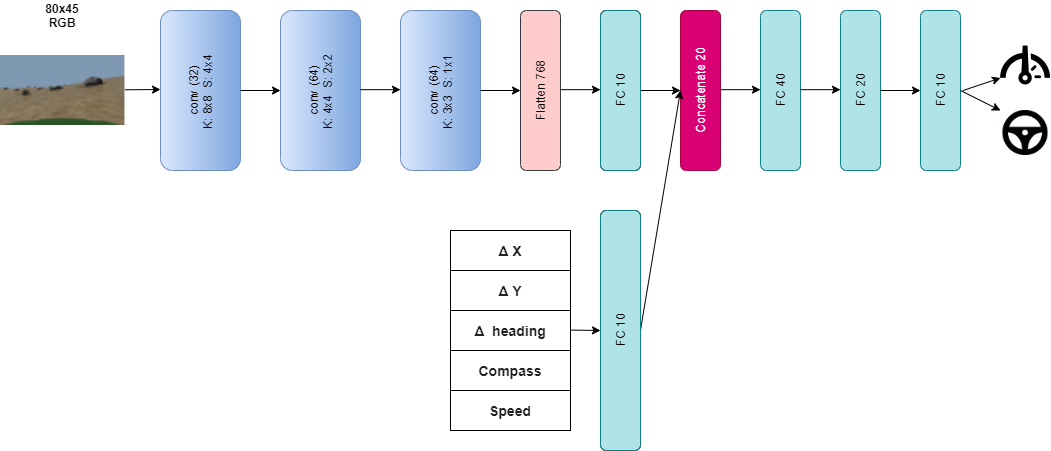
\includegraphics[width=.95\linewidth]{images/CORL_paper_arch.pdf}
    \caption{Actor neural network architecture}
    \label{fig:NN_arch}
\end{figure}


%local vs global (from GPS)


Given the GPS coordinates of the vehicle and the goal, along with the orientation of the vehicle from the IMU, it is straightforward (for a human) to evaluate the distance between the vehicle and the objective. This being said, there are several ways to pass this information to the NN as an input: directly feeding the GPS coordinates, the coordinate difference, the relative distance in a frame oriented along the cardinal points or the distance in the local frame of the vehicle. The last is obviously the most meaningful information but we might want to use coarser inputs and leave to the optimization to infer the correlation. This approach, however, would be inefficient as shown in Fig. \ref{fig:plotLocGlob}, where is clearly shown the benefit, in terms of convergence, of simply rotating the position of the goal with respect to the vehicle in the vehicle reference frame (called \emph{local}).


\begin{wrapfigure}{r}{0.50\textwidth}
    \vspace{-25pt}
    \begin{center}
        \includegraphics[width=.90\linewidth]{images/rewards_localglobal.pdf}
        \caption{On flat terrain without obstacles, the algorithm converges immediately when feeding the position of the goal rotated in the vehicle reference frame. When the position is given in the global frame, training does not converge.}
        \label{fig:plotLocGlob}
    \end{center}
    \vspace{-15pt}
\end{wrapfigure}We adopted a curriculum learning approach \cite{BengioCurriculumLearning09}, progressively increasing the complexity of the task, as shown in Fig. \ref{fig:rew_progr}. The first part of the training was performed on flat terrain with a random number of obstacles (from 0 to 30). After $\sim$ 200 policy updates, when the convergence is reached, the obstacle number is fixed at 30, and after a drop off the convergence is reached again quickly. When, after 376 policy updates, the flat terrain is replaced with hilly terrain (while keeping the same number of obstacles), the agent struggles and many updates are required in order to converge again. In the third and last stage of the training, the obstacle count was increased to 50 and the terrain texture was randomized. Curriculum learning was deemed necessary when convergence could not be directly reached from scratch on hilly terrain. Moving through multiple training approaches, we found that: ($i$) Irregularities in terrain height cause policies trained exclusively on flat terrains to perform poorly; ($ii$) This problem can by solved by undergoing further training on hilly terrain; and, ($iii$) The curriculum learning approach (see Fig.~\ref{fig:rew_progr}) was instrumental in eventually handling the complex tasks; i.e., hills with many random obstacles.


% distributed training, batch and minibatch size, Adam with HP, 
Training relied on the ADAM algorithm \cite{Kingma14ADAM} with a learning rate of 1e-4. The training set at each update included 6000 tuples (timesteps), fed by 1000 element mini-batches to the optimizer, which operated eight epochs per update.
Since Chrono is compatible with OpenAI gym \cite{Brockman16Gym} environments, the dataset was collected by running six parallel episodes leveraging OpenAI baselines \cite{baselines} multiprocessing tools.
% MB size comment?
\begin{figure}[h]
    \centering
    \includegraphics[width=.75\linewidth]{images/CORLrewards.pdf}
    \caption{Reward progression. Vertical lines represent the changes introduced to make the environment more challenging. In order of occurrence, the dotted lines mark: fix obstacle count at 30; change from flat to hilly terrain; and increase of obstacle count to 50. }
    \label{fig:rew_progr}
\end{figure}


%!TEX root = ../main.tex
\section{Simulation Experiments}
\label{sec:demoTechnology}
To demonstrate and analyze the capabilities of the control policy, we used an 80$ \times $80 m patch of terrain. The reduced scale of the test environment allowed for rapid evaluation and inclusion of tests using deformable terrain based on the Soil Contact Model (SCM) \cite{ChronoSCM2019}. For all tests, the vehicle is placed at world location (-35,35); to be successful, it must navigate safely to within a 10 m radius of world location (35,-35). This setup was a matter of convenience and is not a limitation of the policy. Since training used a larger patch of 120$ \times $120 m, it is important to note that parameters such as number of obstacles and height of terrain cannot be compared directly with testing; this was done on purpose. For the terrain patch, and equivalent number of obstacles to the 50 used in training is approximately 22. Additionally, the maximum height difference of 10 m in training is equivalent to a height of approximately 7.25 m on the testing terrain. Furthermore, in testing, to prevent the vehicle from successfully navigating purely along the diagonal straight toward the destination, five obstacles were placed randomly near the diagonal to force non-trivial trajectories. Overall, the tests were conducted with a higher-complexity environment that used in training. They were designed to probe the robustness of the algorithm and understand to what extent the policy could be used on never-before-seen terrain. We looked at ($i$) increased levels of hilliness; ($ii$) increased number of obstacles; and ($iii$) alterations of the soil including rigid, hard-deformable (silt-like), and soft-deformable (snow-like). 

Figure \ref{fig:scm_soft_hilly_deformed} shows a snapshot of one scenario: the soft deformable terrain used for testing robustness; a capture of the image from the camera sensor used by the NN; and the position of the vehicle along its current trajectory with the obstacles and height map overlaid for context (height map: black is valleys, white is peaks). 

\begin{figure}[h]
    \centering
    \includegraphics[height=.1095\paperheight]{images/demonstration/scm_soft_hilly_montage_final.png}
    \caption{Snapshot of a scenario used for testing. Left: third-person perspective of the vehicle; center: image from the camera's view at the resolution used in training 80$ \times $45 pixels; right: the current progress of the vehicle amount the hills and obstacles corresponding to the images on left. }
    \label{fig:scm_soft_hilly_deformed}
\end{figure}

Figure \ref{fig:example_paths} shows an example set of paths navigated by the Gator in the test environment. In Fig. \ref{fig:rigid_flat_3_example12}, the vehicle avoids a sparse environment, limited to 20 obstacles. By increasing the obstacles to 50, as shown in Fig. \ref{fig:rigid_flat_9_example22}, the complexity of the test environment forces the policy into a correspondingly complex path. An example failure is illustrated in Fig. \ref{fig:rigid_flat_9_failure_example0} where the vehicle does not reach the destination owing to a collision. Any scenario where the vehicle collides with an obstacle is deemed a failure, regardless of how directly the vehicle collides with the obstacle. The last example, shown in Fig. \ref{fig:rigid_height_map_example13}, demonstrates the vehicle navigating a hilly terrain, created from a programmatically generated random height map.


\begin{figure}[h]
    \captionsetup{justification=centering}
    \centering
    \begin{subfigure}{0.24\textwidth}
        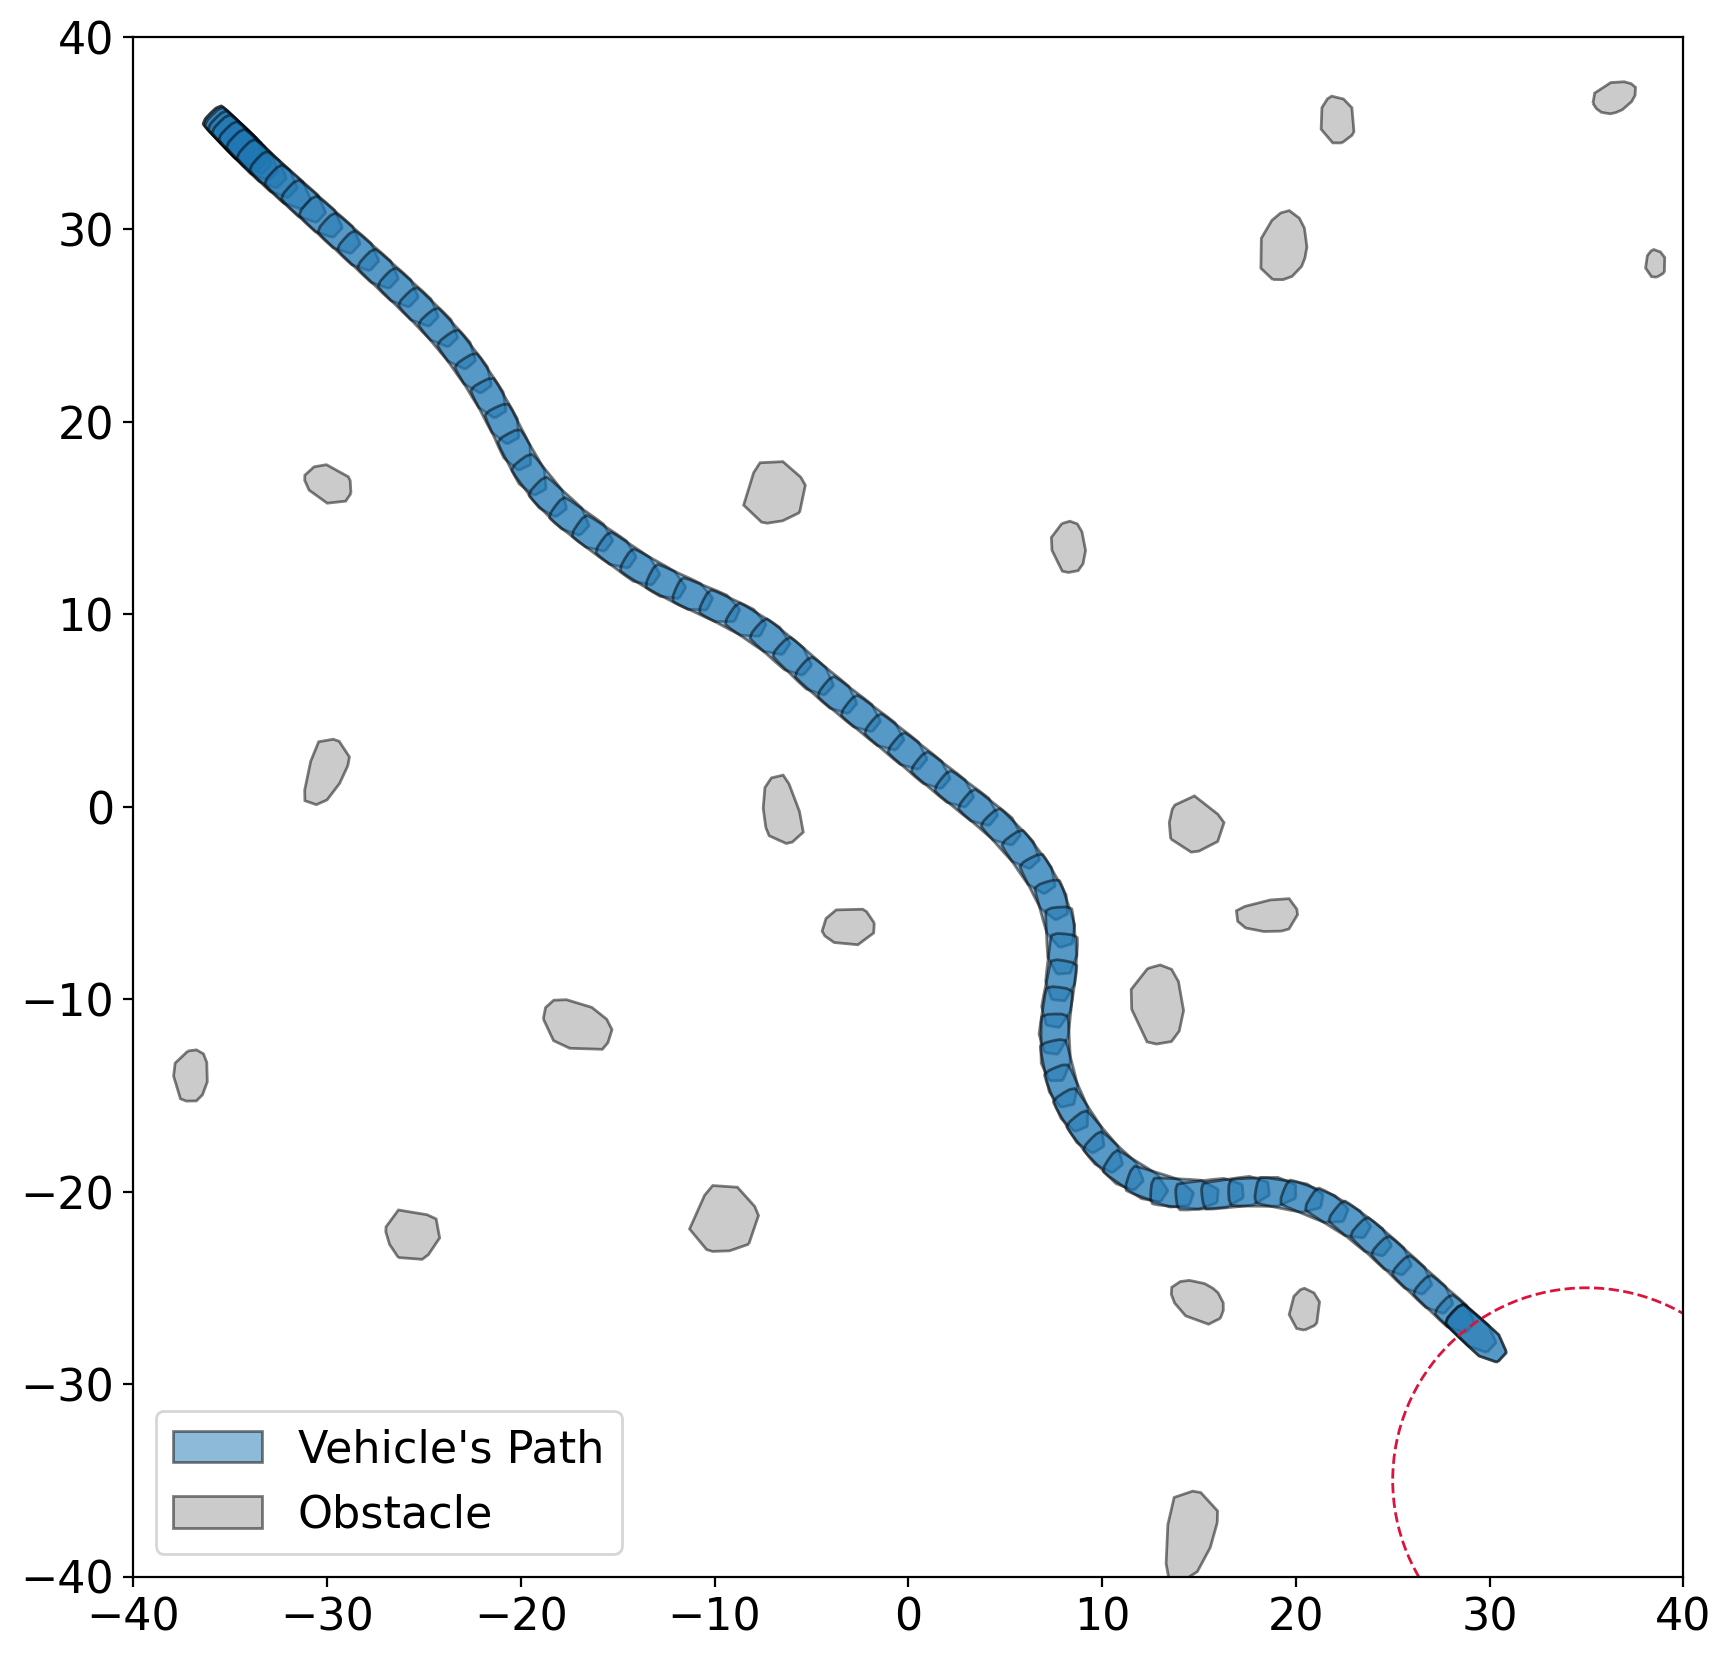
\includegraphics[height=.12\paperheight]{images/demonstration/rigid_flat_3_example12.png}
        \caption{}
        \label{fig:rigid_flat_3_example12}
    \end{subfigure}
    \hfill
    \begin{subfigure}{0.24\textwidth}
        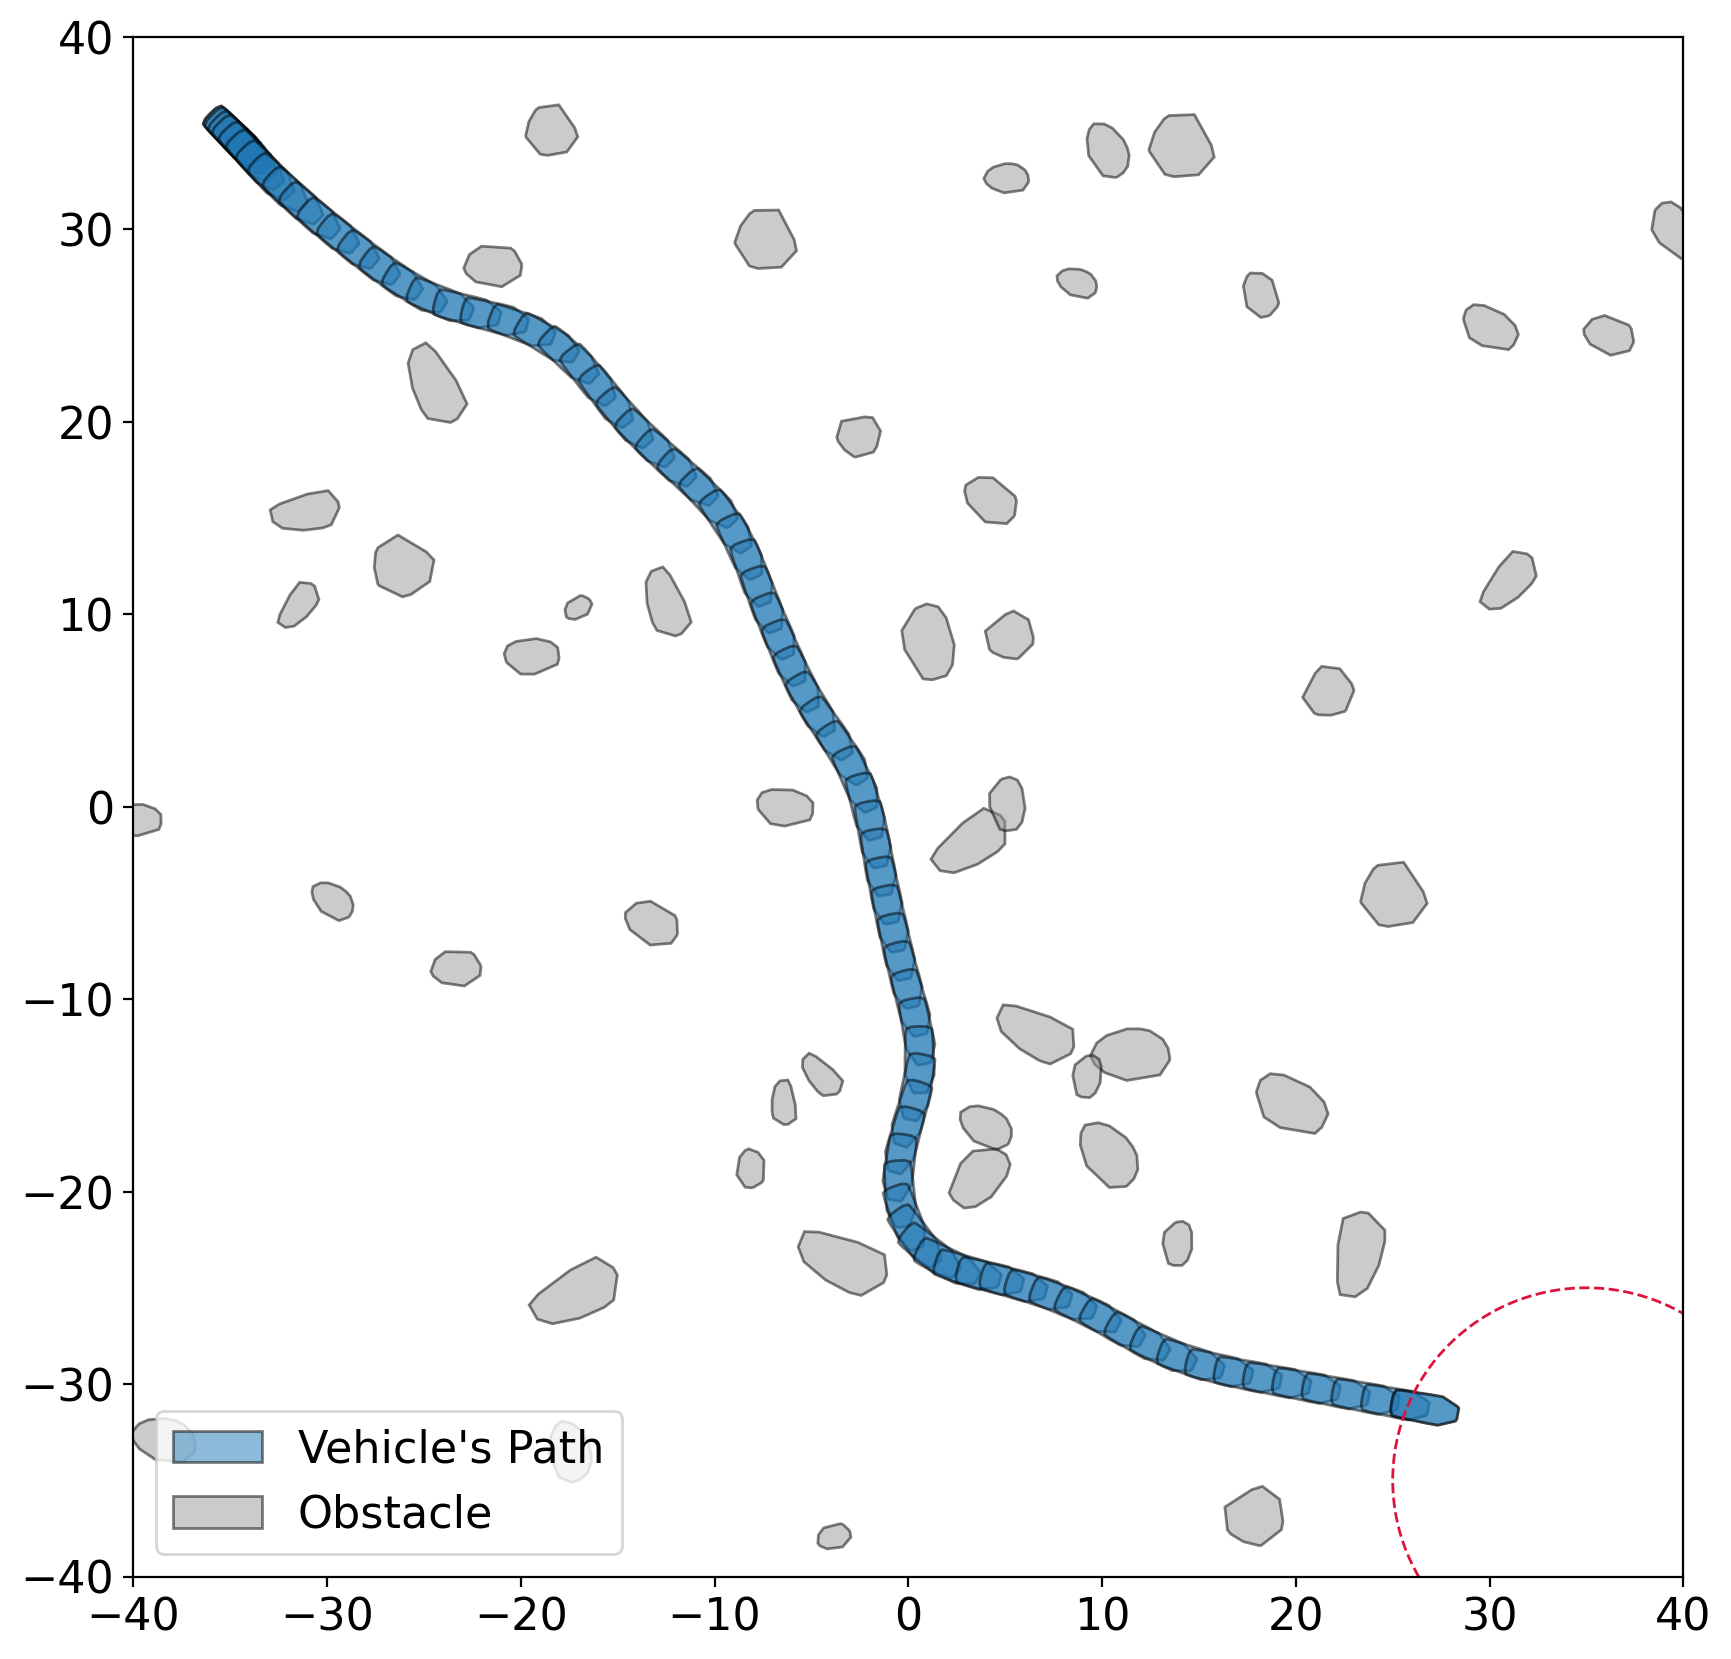
\includegraphics[height=.12\paperheight]{images/demonstration/rigid_flat_9_example22.png}
        \caption{}
        \label{fig:rigid_flat_9_example22}
    \end{subfigure}
    \hfill
    \begin{subfigure}{0.24\textwidth}
        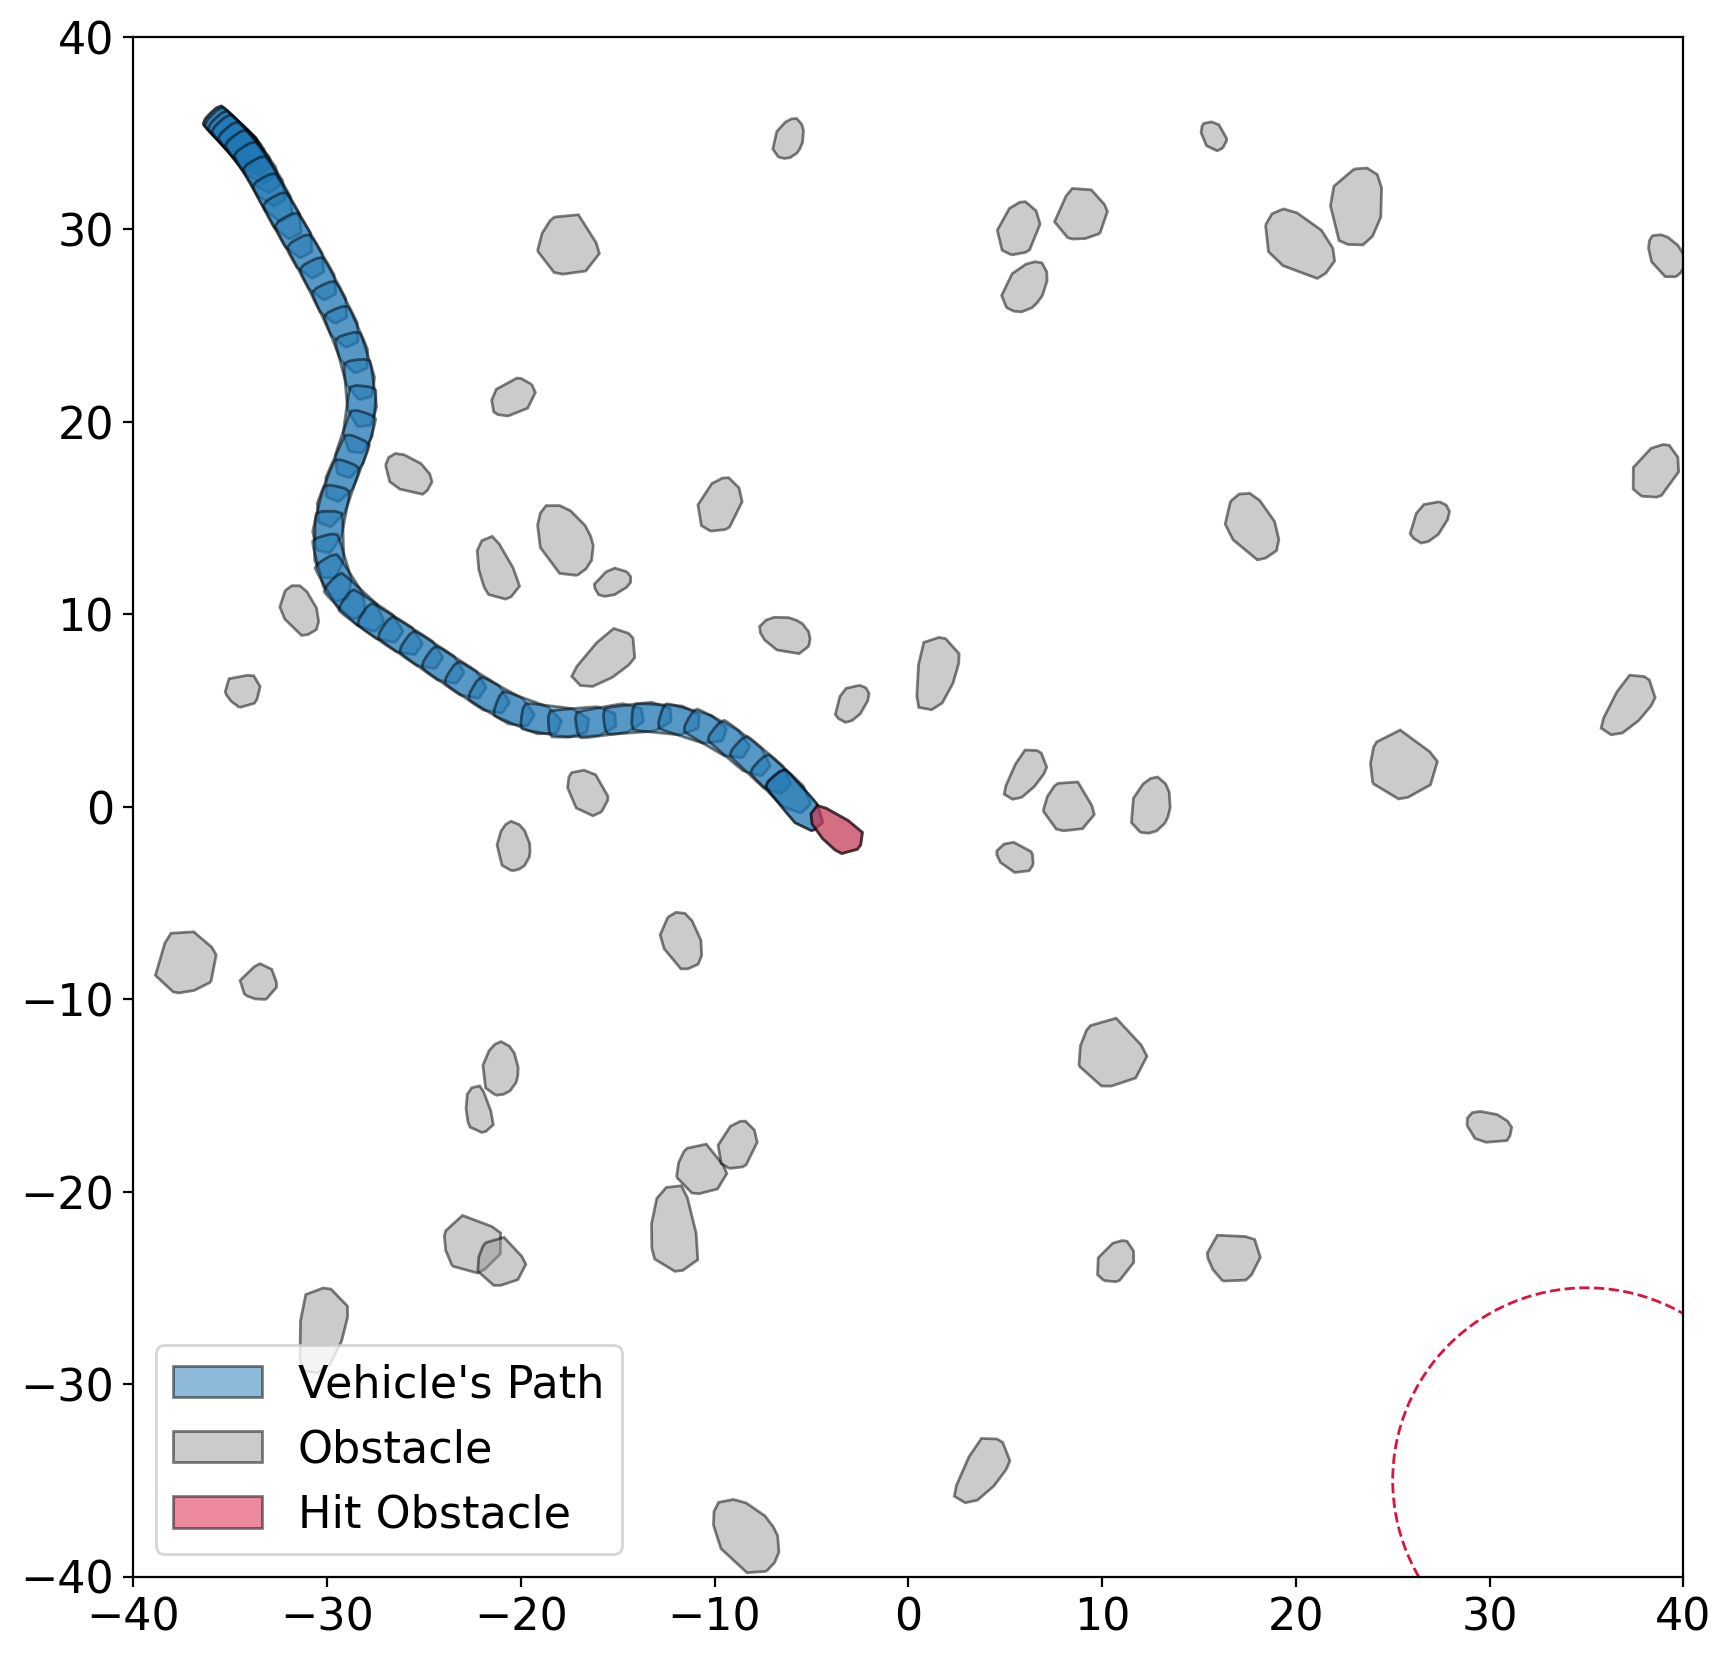
\includegraphics[height=.12\paperheight]{images/demonstration/rigid_flat_9_failure_example0.png}
        \caption{}
        \label{fig:rigid_flat_9_failure_example0}
    \end{subfigure}
    \hfill
    \begin{subfigure}{0.24\textwidth}
        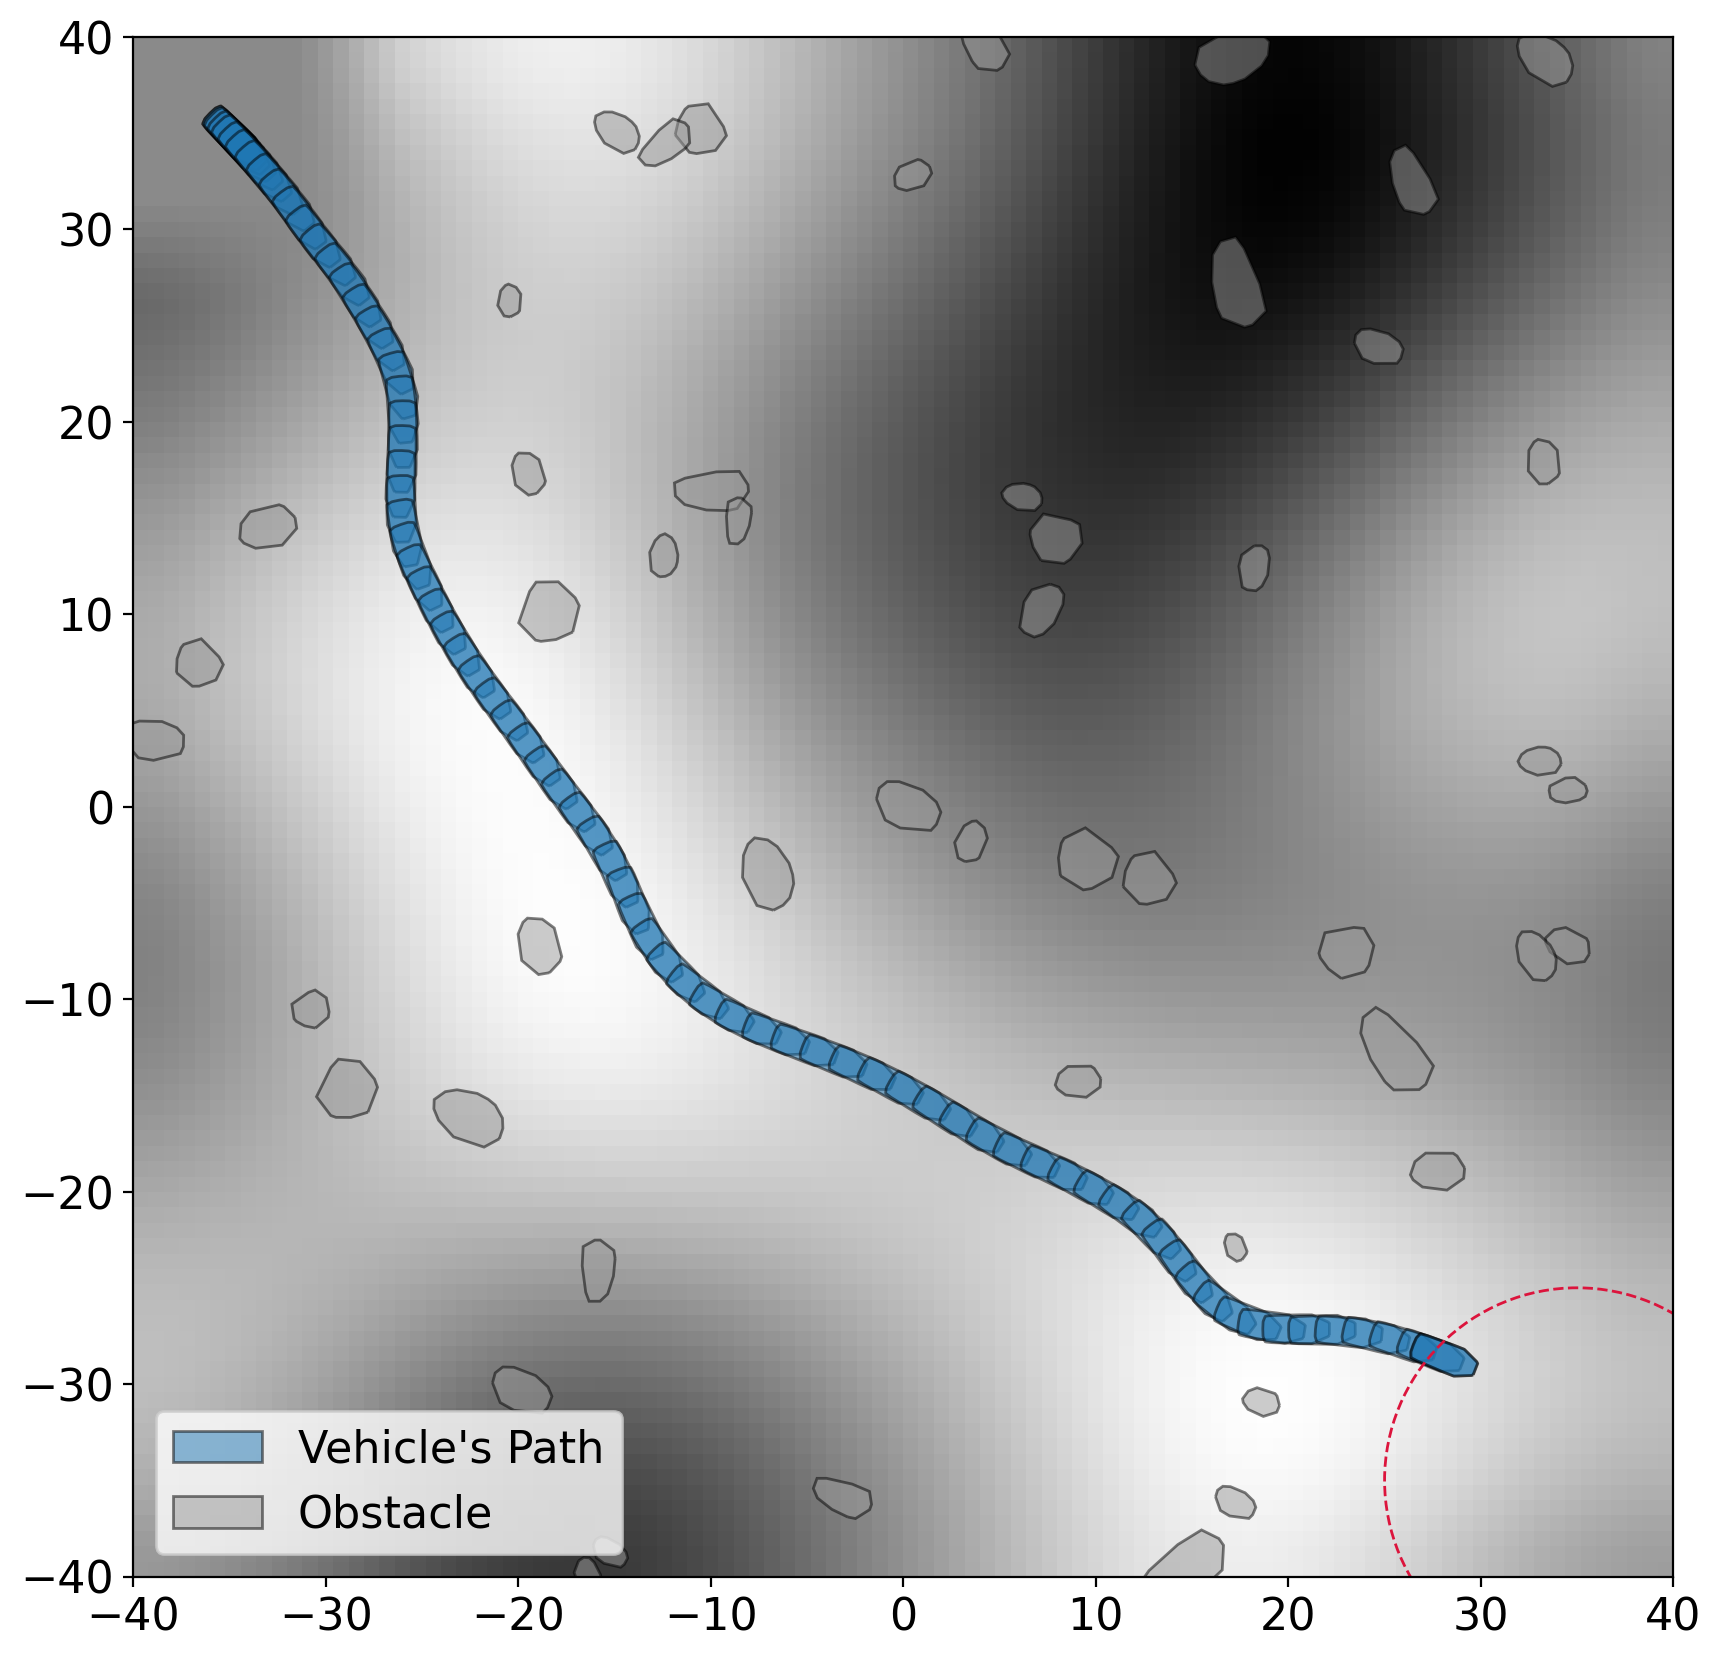
\includegraphics[height=.12\paperheight]{images/demonstration/rigid_height_map_example13.png}
        \caption{}
        \label{fig:rigid_height_map_example13}
    \end{subfigure}
    \caption{Example test scenarios: (a) 20 obstacles, (b) 50 obstacles, (c) failure with 50 obstacles, (d) hilly terrain with 50 obstacles.}
    \label{fig:example_paths}
\end{figure}

In an attempt to assess the practicality of the vehicle's chosen path, a Particle Swarm Optimization (PSO) algorithm \cite{PSOObstacleAvoidance} with global knowledge of the environment was used to generate reference trajectories in the environment; they were used in post-processing only, for comparison purposes. Figure \ref{fig:rigid_flat_pso_example3} shows a comparison between the trained vehicle's path and a trajectory generated using the PSO path planner. In this example, 40 obstacles are present on rigid, flat terrain. %What would have been undesirable to see was that the trained vehicle skirted the edges of the domain or assumed unreasonable trajectories. This turned out to not be the case.

\begin{figure}[h]
    \captionsetup{justification=centering}
    \centering
    \begin{subfigure}{0.329\textwidth}
        \centering
        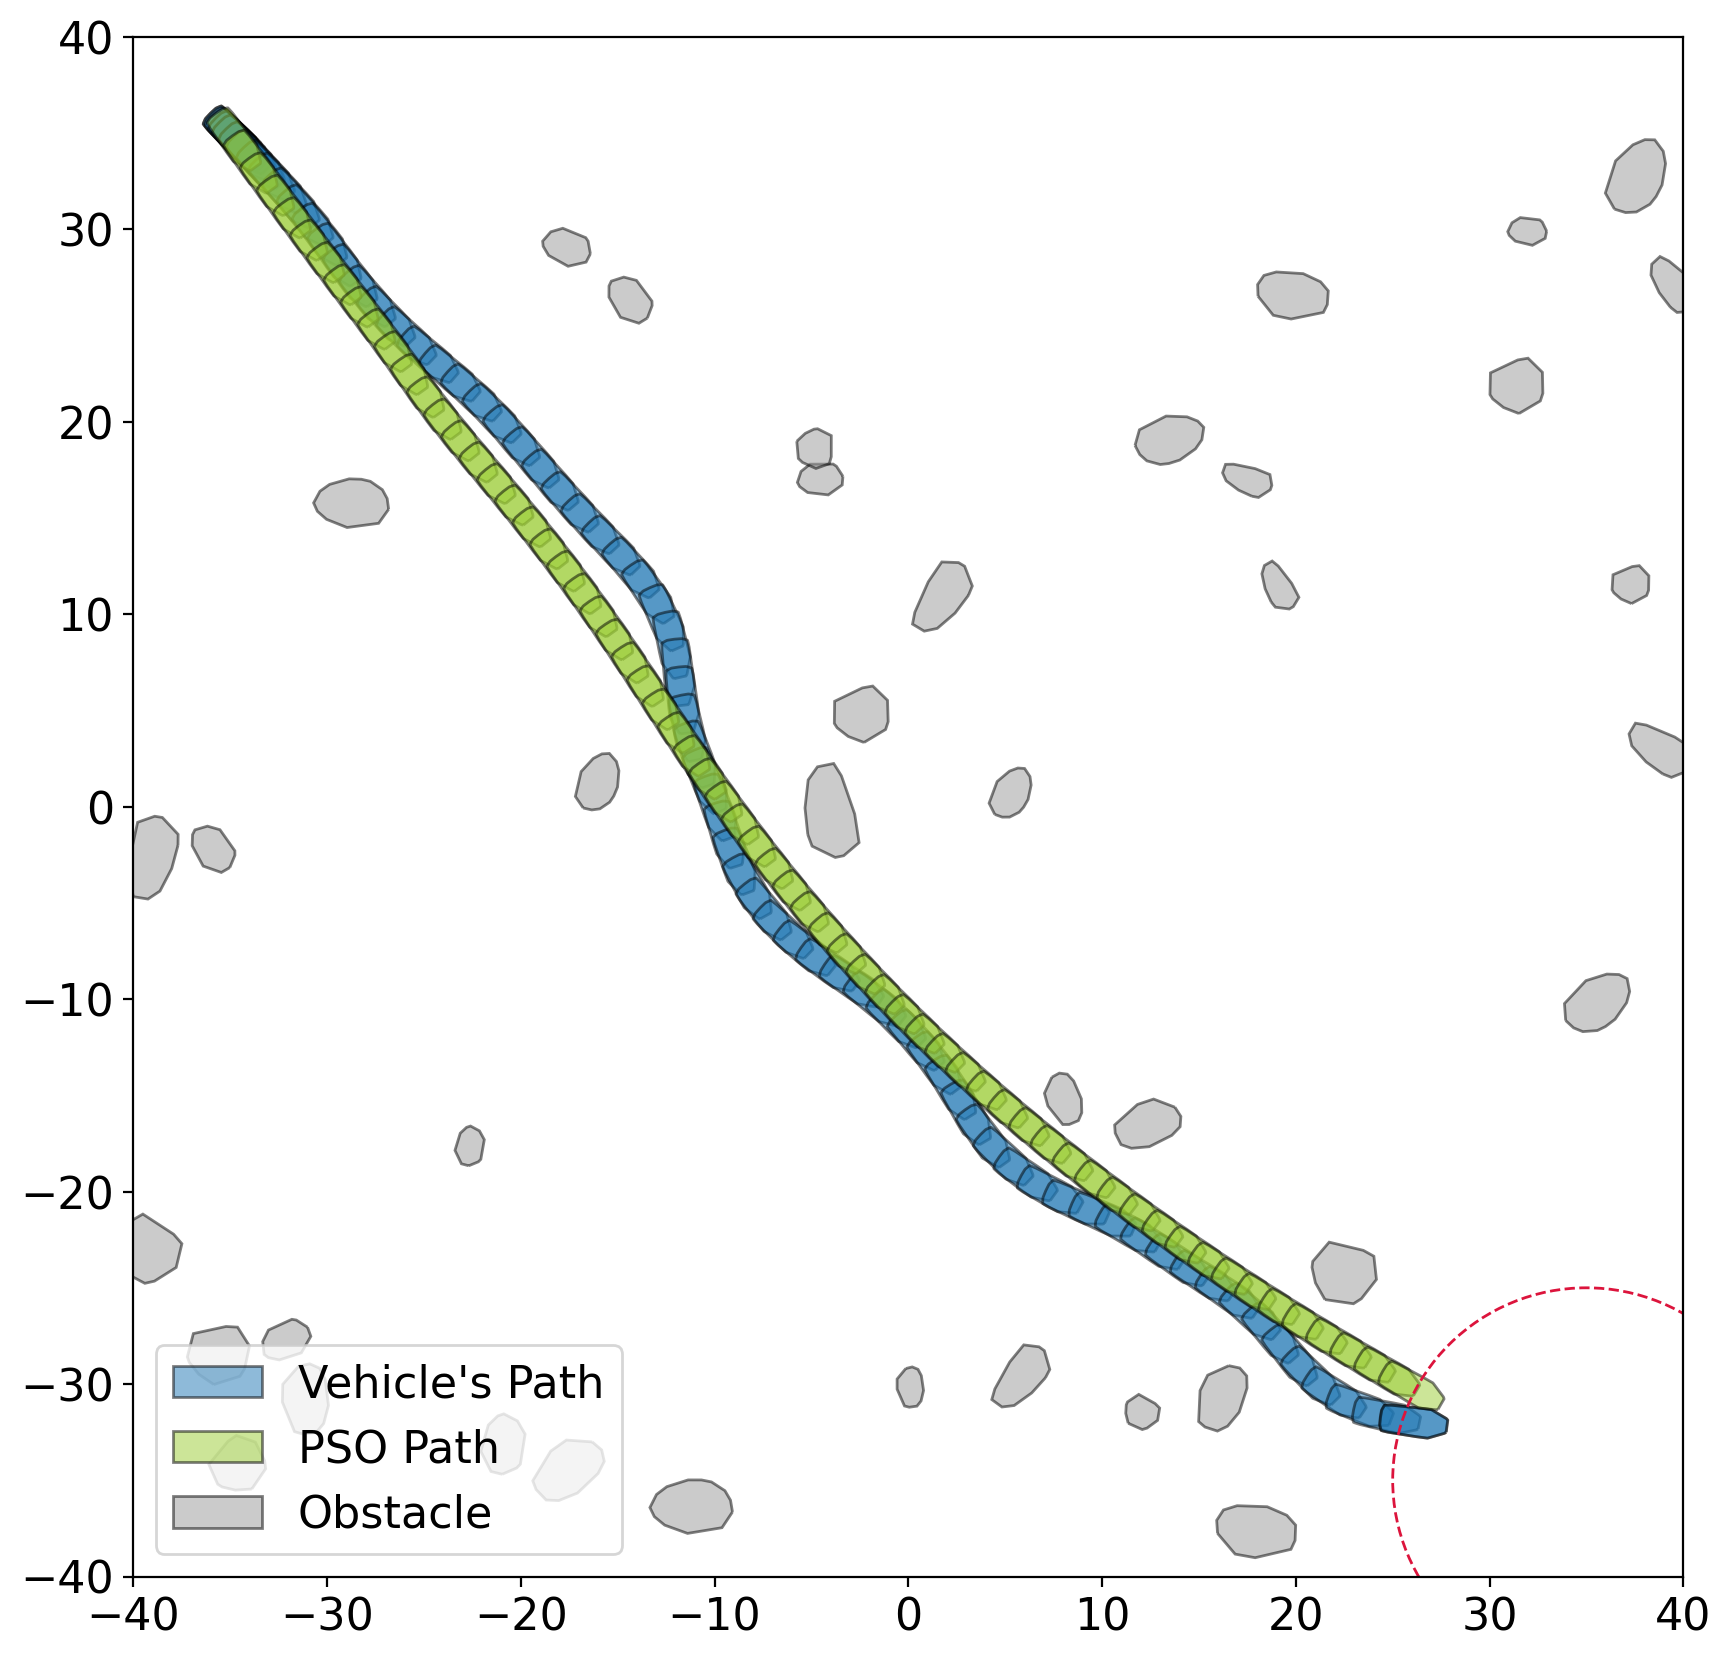
\includegraphics[height=.155\paperheight]{images/demonstration/rigid_flat_pso_example3.png}
        \caption{Example comparison between the Gator's path and PSO path.}
        \label{fig:rigid_flat_pso_example3}
    \end{subfigure}
    \hfill
    \begin{subfigure}{0.329\textwidth}
        \centering
        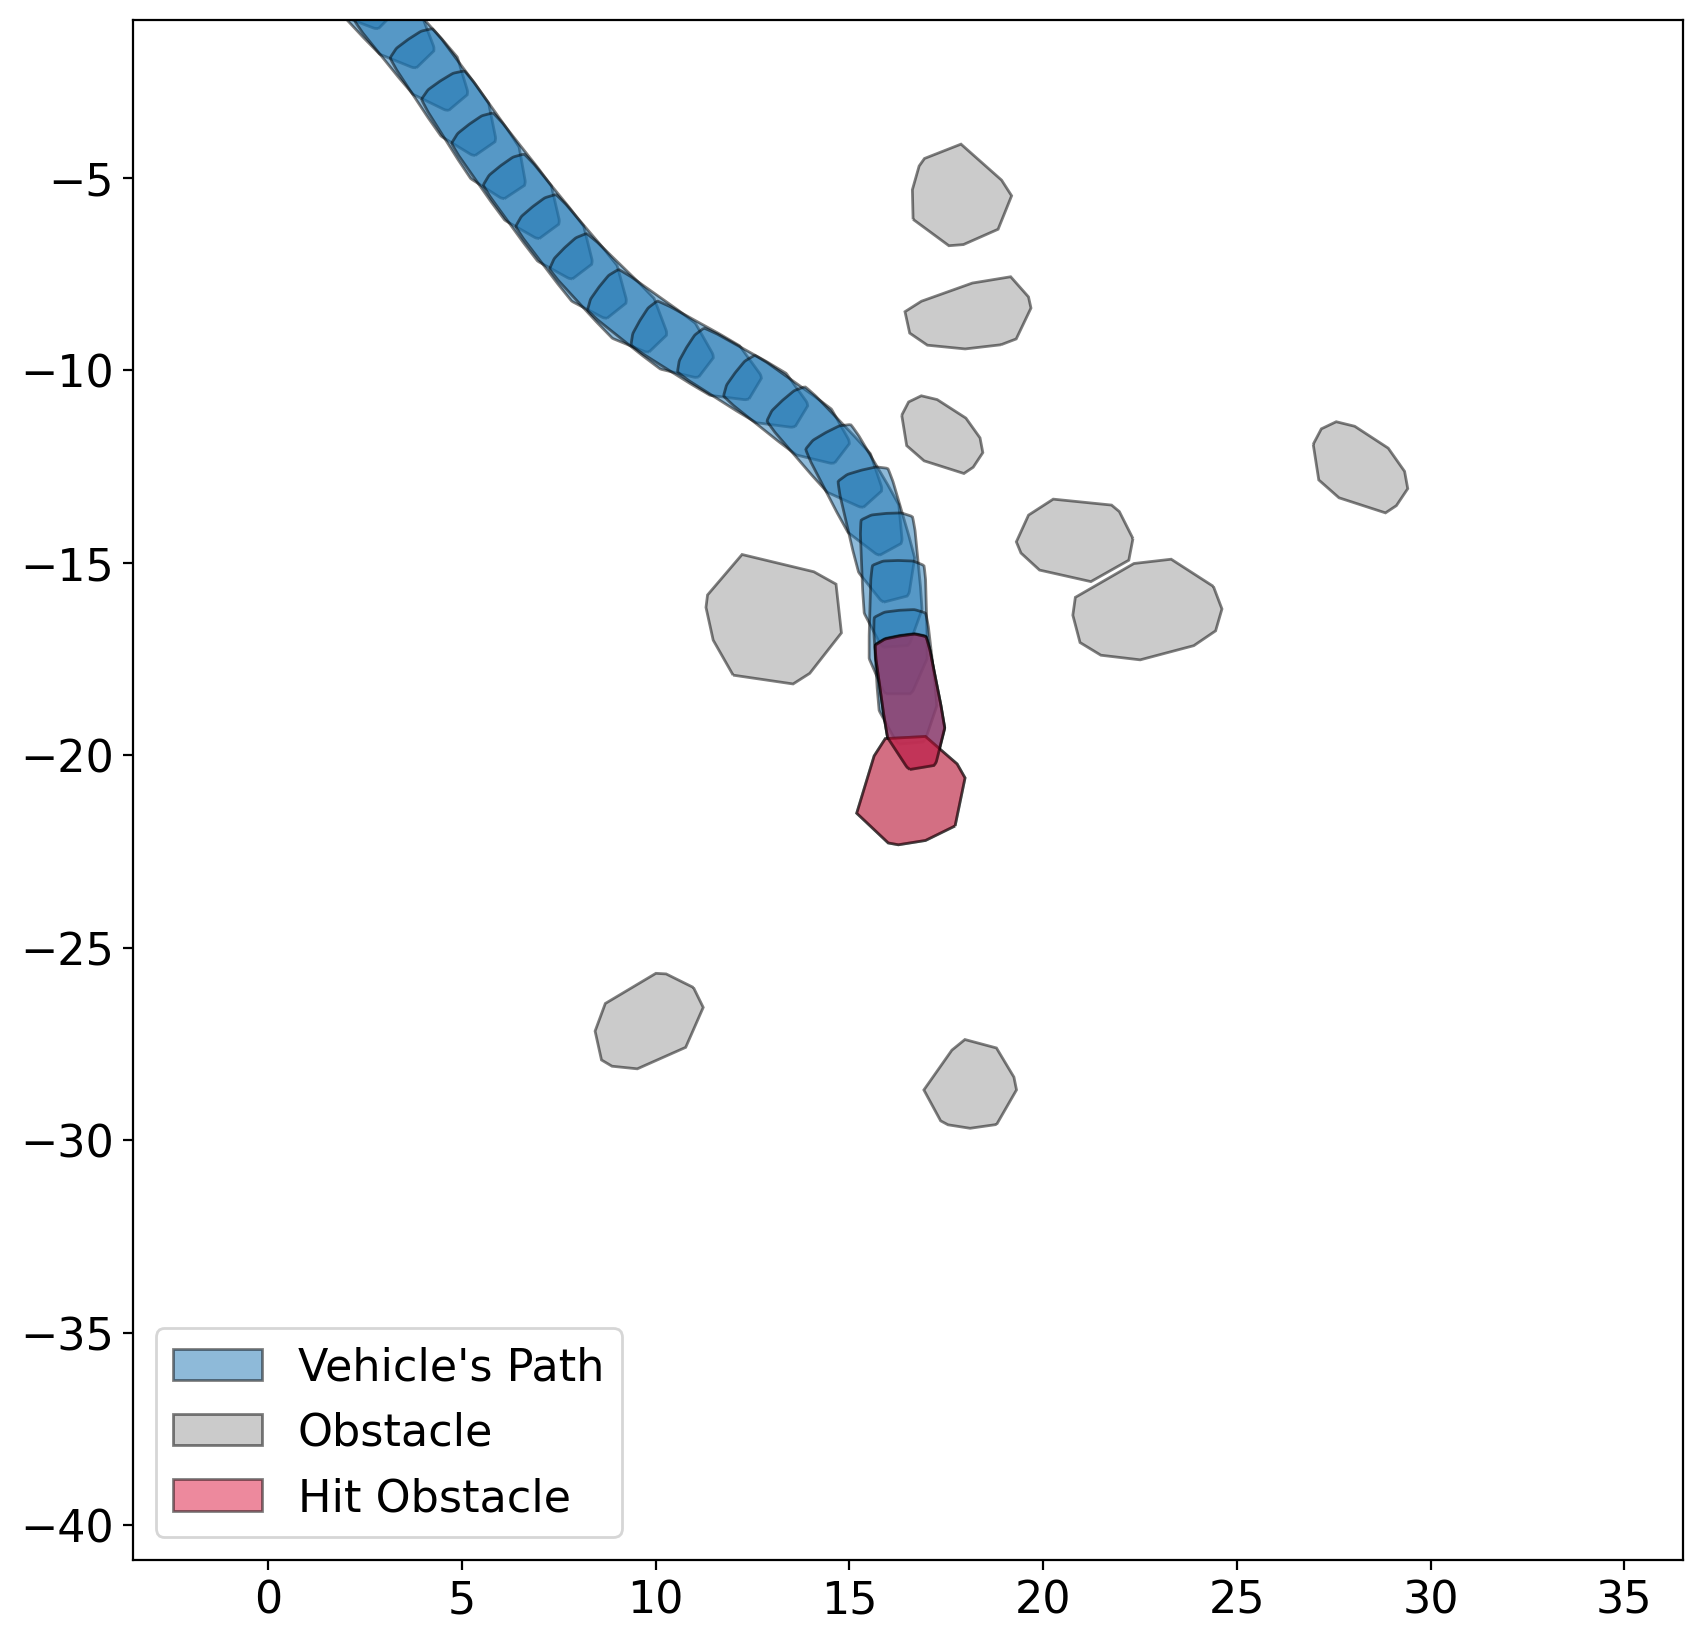
\includegraphics[height=.155\paperheight]{images/demonstration/rigid_40_failure_100.png}
        \caption{Example collision where the directness of the impacts was 100\%.}
        \label{fig:rigid_40_failure_100}
    \end{subfigure}
    \hfill
    \begin{subfigure}{0.329\textwidth}
        \centering
        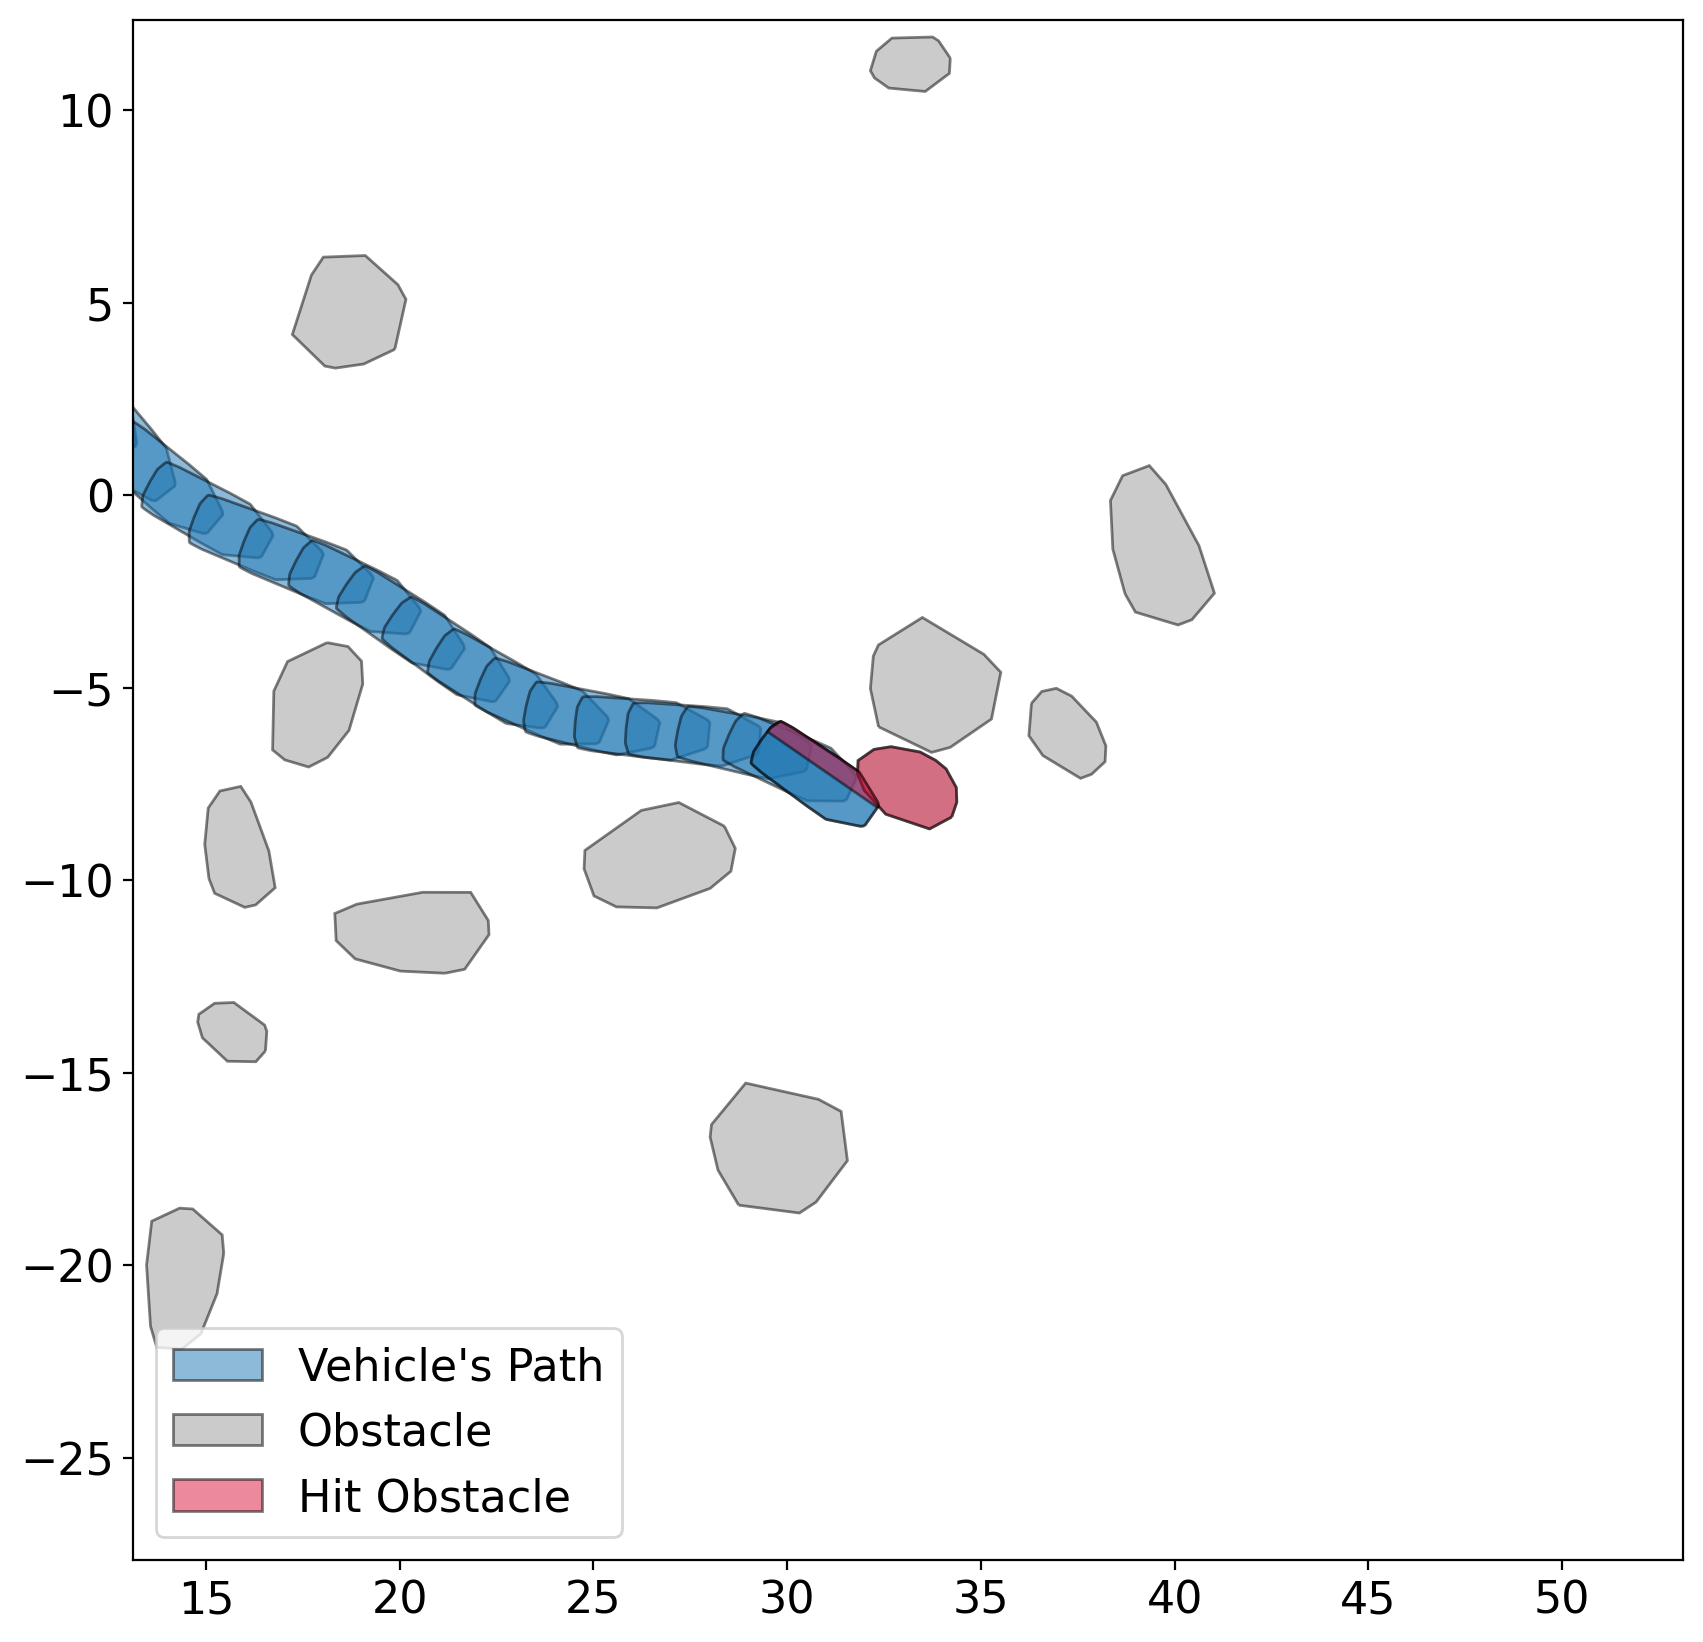
\includegraphics[height=.155\paperheight]{images/demonstration/rigid_40_failure_34.png}
        \caption{Example collision where the directness of the impacts was 34\%.}
        \label{fig:rigid_40_failure_34}
    \end{subfigure}
    \caption{Example paths showing comparison with global path planner and two levels of collision directness.}
\end{figure}


%%!TEX root = ../main.tex
%
%
%\section{Results}

To quantify the end-to-end learned navigation, the primary metric is success rate. This is simply a measure of the vehicle's ability to reach the destination without colliding with any obstacles. For this metric, any collision, regardless of severity, is considered a failure and the simulation is terminated. In addition to the primary metric, the length of the path is analyzed relative to the PSO path. Since the PSO path would generally be able to find a shorter path than the trained algorithm, which only has local information, the comparison will be used to show that the path taken by the trained algorithm is reasonable, and not simply a path that avoids obstacles yet produces bizarre trajectories.

When testing the effect of hilliness on navigation, the maximum height of the random height map was increased from 0 m (flat) to 12 m in increments of 2 m. At each level, 200 simulations on random height maps generated using simplex noise were performed to understand the success rate of the algorithm with respect to the terrain change. The results are shown in Fig. \ref{fig:rigid_height_success}. As expected, the trained network's ability to safely navigate the environment decreases with increased hilliness. Additionally, as the number of obstacles is increased, the task becomes more difficult. Tests conducted with 20 obstacles represent the closest point to the training environment.

In addition to the increasing height tests, experiments were conducted with hilliness of 0 m and 6 m with three terrain models: undeformable (rigid), hard-deformable, and soft-deformable. Since no deformable terrain was experienced in training, this is also a measure of policy robustness with respect to the terrain. These results, for varying terrain, heights, and obstacles are shown in Fig. \ref{fig:obstacles_hilly_and_flat_success}. While the policy can maintain relatively high success on deformable soil when the terrain is flat, the combination of deformable and hilly terrain proves difficult for the policy with success rates falling below 50\%.

\begin{figure}
    \captionsetup{justification=centering}
    \centering
    \begin{subfigure}{0.36\textwidth}
        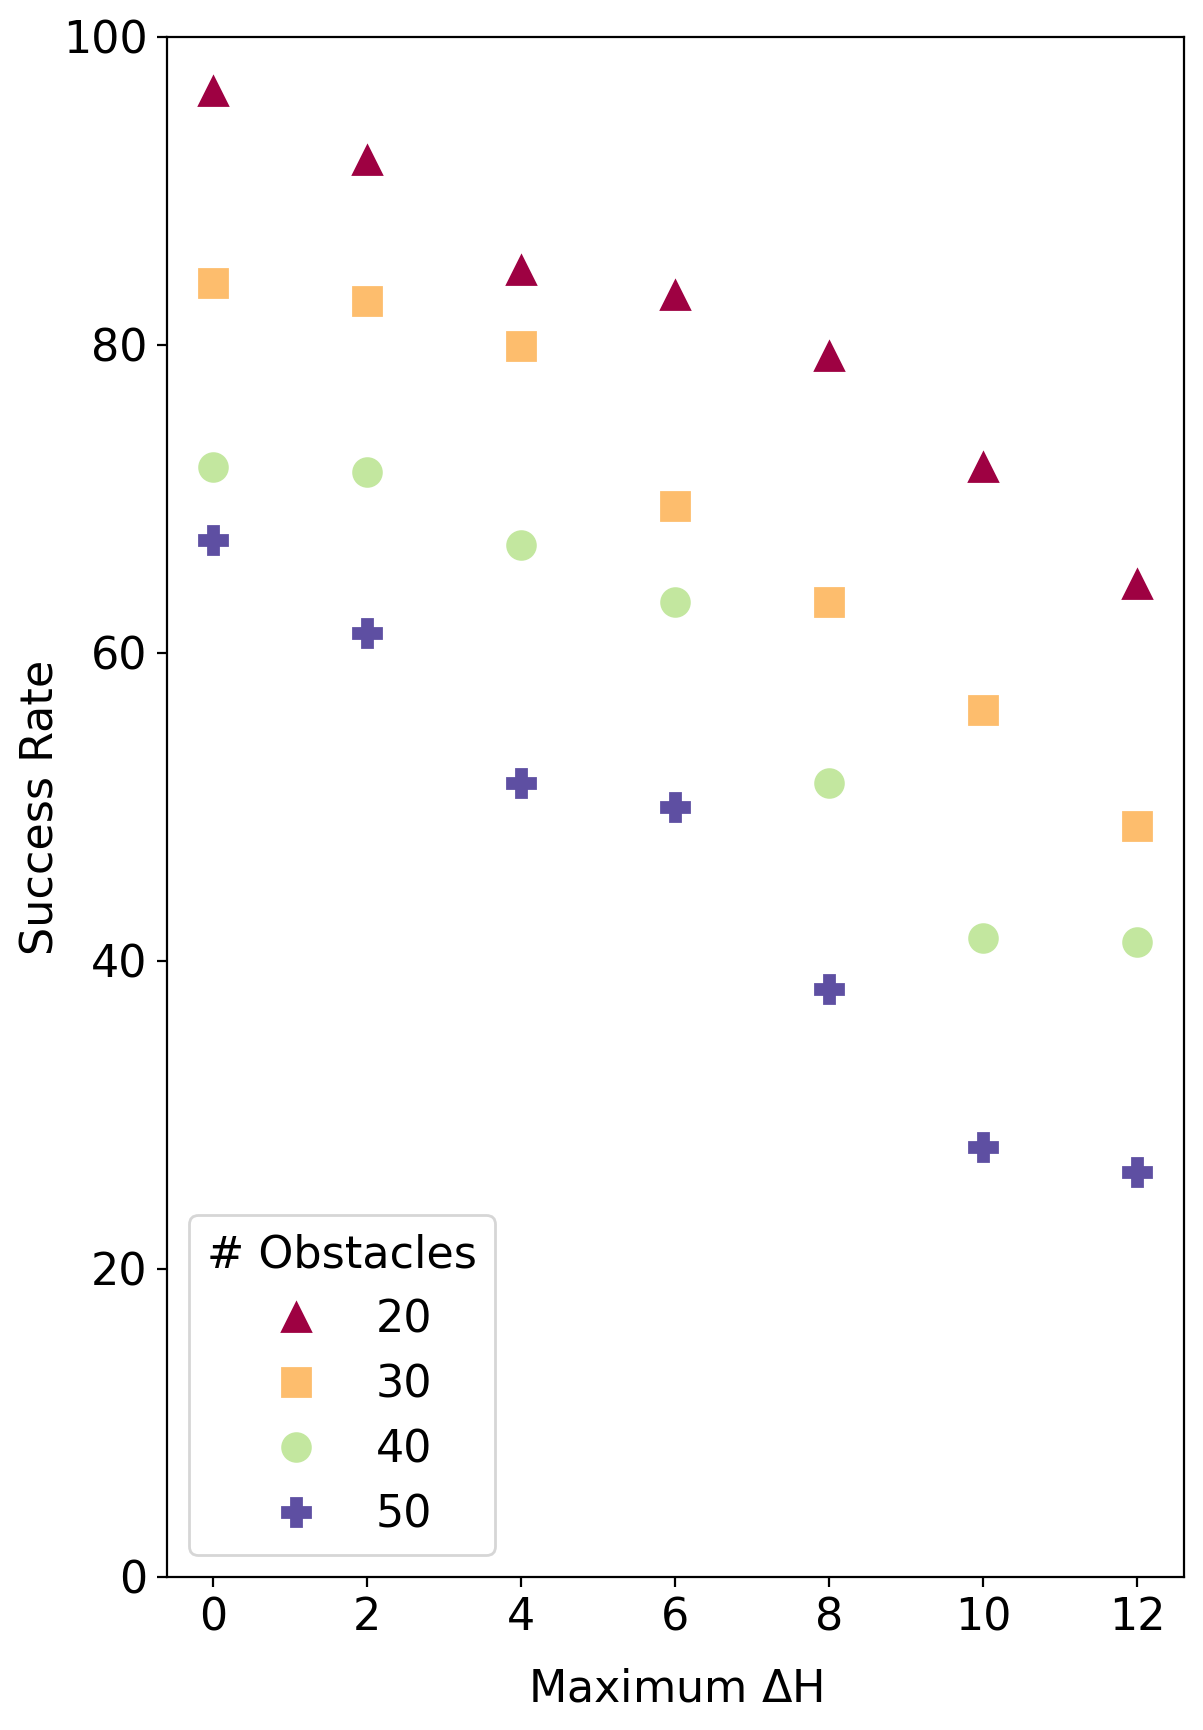
\includegraphics[height=.25\paperheight]{images/demonstration/rigid_height_success_rate.png}
        \caption{Success rate in \% vs hilliness on rigid terrain.}
        \label{fig:rigid_height_success}
    \end{subfigure}%
    \hfill
    \begin{subfigure}{0.44\textwidth}
        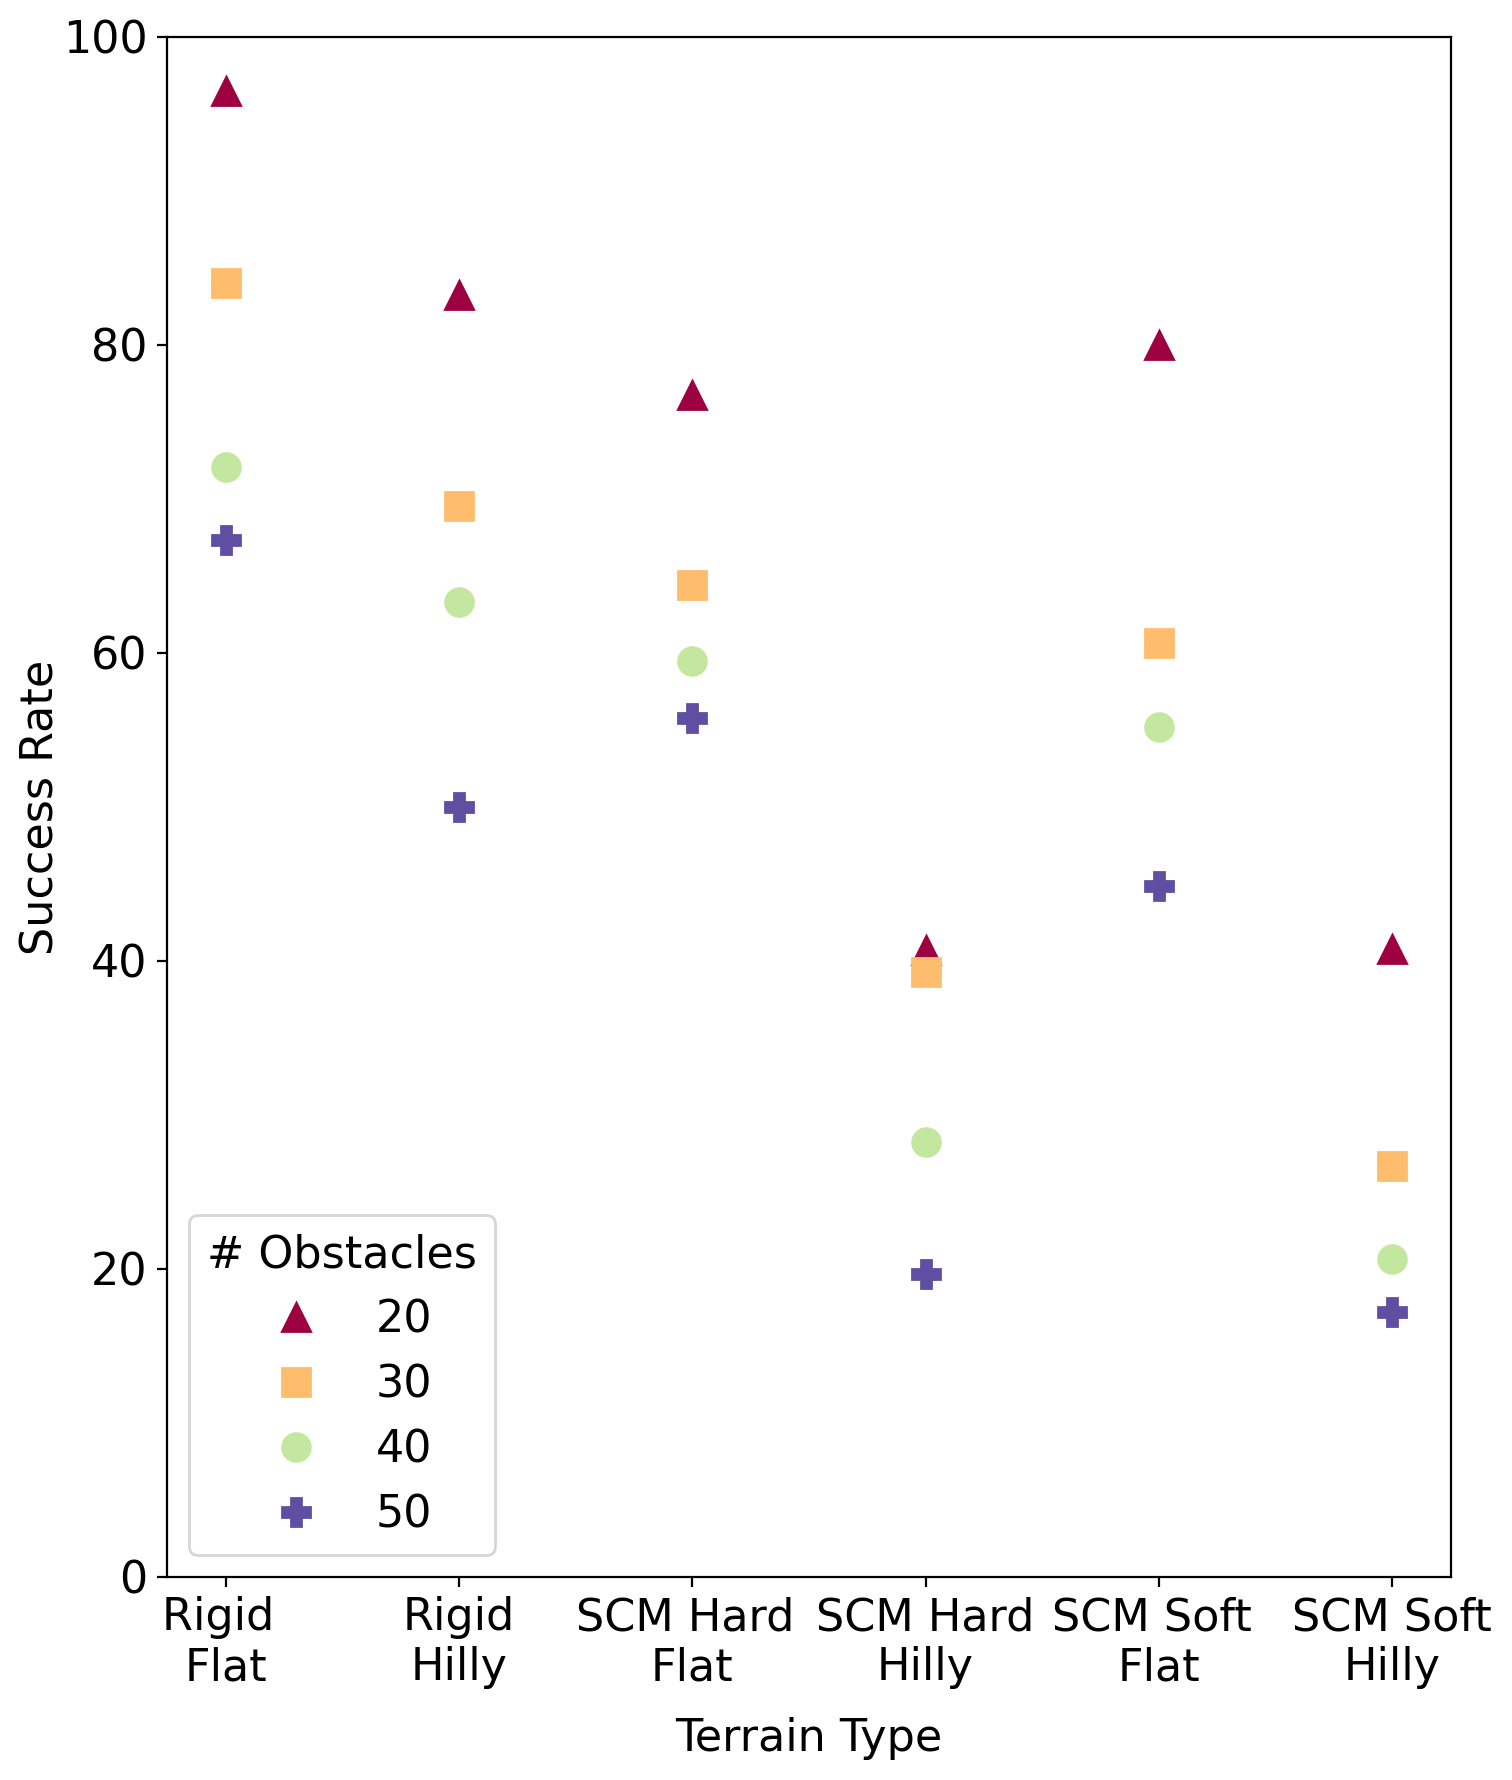
\includegraphics[height=.25\paperheight]{images/demonstration/terrain_obstacles_flat_and_height_success_rate.png}
        \caption{Success rate in \% vs hilly and flat terrains with varying stiffness.}
        \label{fig:obstacles_hilly_and_flat_success}
    \end{subfigure}
    \caption{Success rate when increasing complexity of the terrain.}
    \label{fig:successRates}
\end{figure}

The second metric, which compares the length of the chosen path to the length of a path generated by the PSO, is discussed for a single environment setup. This is shown in Fig. \ref{fig:pso_length_compare} for flat, rigid terrain with 50 obstacles, which is more than double the obstacle density used in training. The length difference is computed as $length(NN path) - length(PSO path)$. These results show that the mode of the distribution is around -5 m, meaning the NN path is most often 5 m longer than the PSO path. While a direct comparison is not feasible since the PSO takes into account global knowledge and does not make any claims about optimality, the path taken by the NN appears to be moderately close in length to a global planner. This means that the policy is appropriately weighting the directness of the path as expected. Only successful paths were included in the calculation of this metric.

To further understand and analyze the success rate of the algorithm, the full set of collisions were evaluated based on the directness of collision. The directness of collision was computed by measuring the overlap of the projection of the vehicle and obstacle onto a plane perpendicular to the vehicle heading. This metric quantifies scraping collisions near 0\% and direct collisions near 100\%. This percentage can be interpreted as the percent of the frontal area of the vehicle that collided with the obstacle. While this cannot directly assign severity to the collision, it can hint at the type of collisions experienced by the policy. The distribution of results in Fig. \ref{fig:rigid_failure_metric_histogram} show that while the mode is near 100\%, there is also a significant portion of the collisions that have low directness. %This suggests that further analysis and adjustments could be made to the training to understand if increased penalty to force the vehicle away from obstacles could improve the success rate further.

\begin{figure}
    \captionsetup{justification=centering}
    \centering
    \begin{subfigure}{0.45\textwidth}
        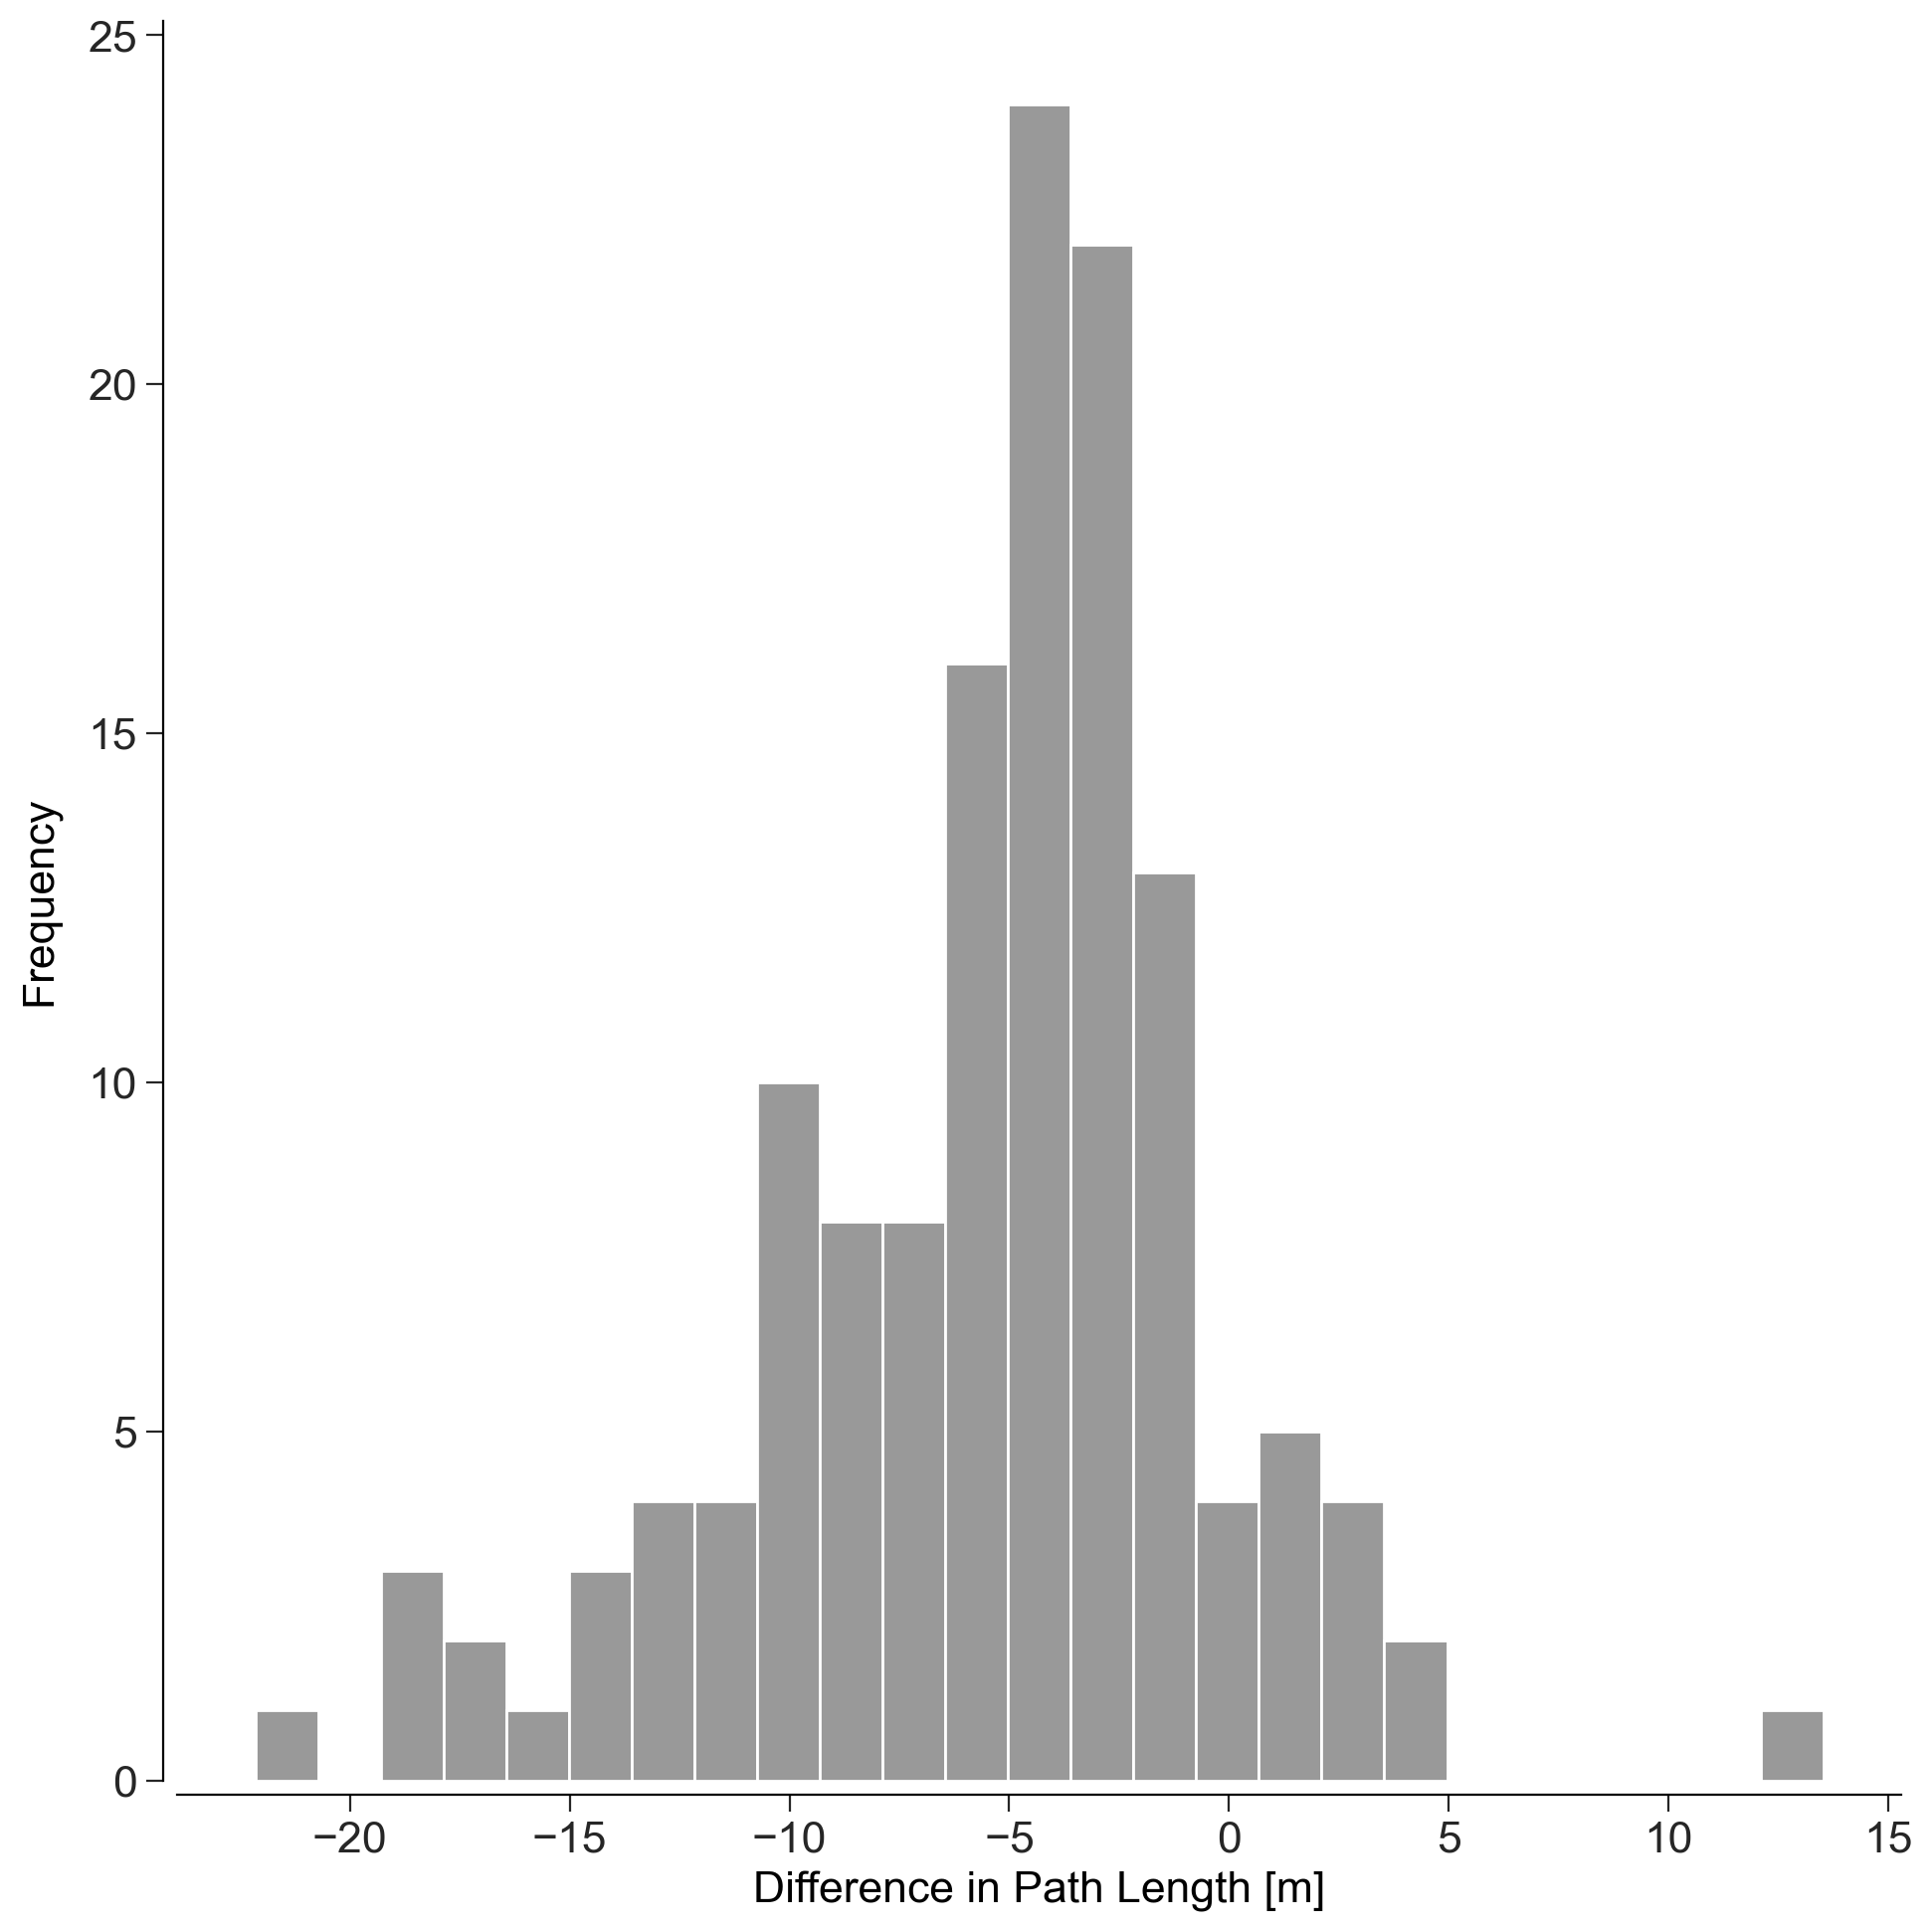
\includegraphics[height=.22\paperheight]{images/demonstration/rigid_9_pso_metric_histogram.png}
        \caption{Difference in path length between the pso trajectory and vehicle path for flat rigid terrain with 50 obstacles.}
        \label{fig:pso_length_compare}
    \end{subfigure}%
    \hfill
    \begin{subfigure}{0.45\textwidth}
        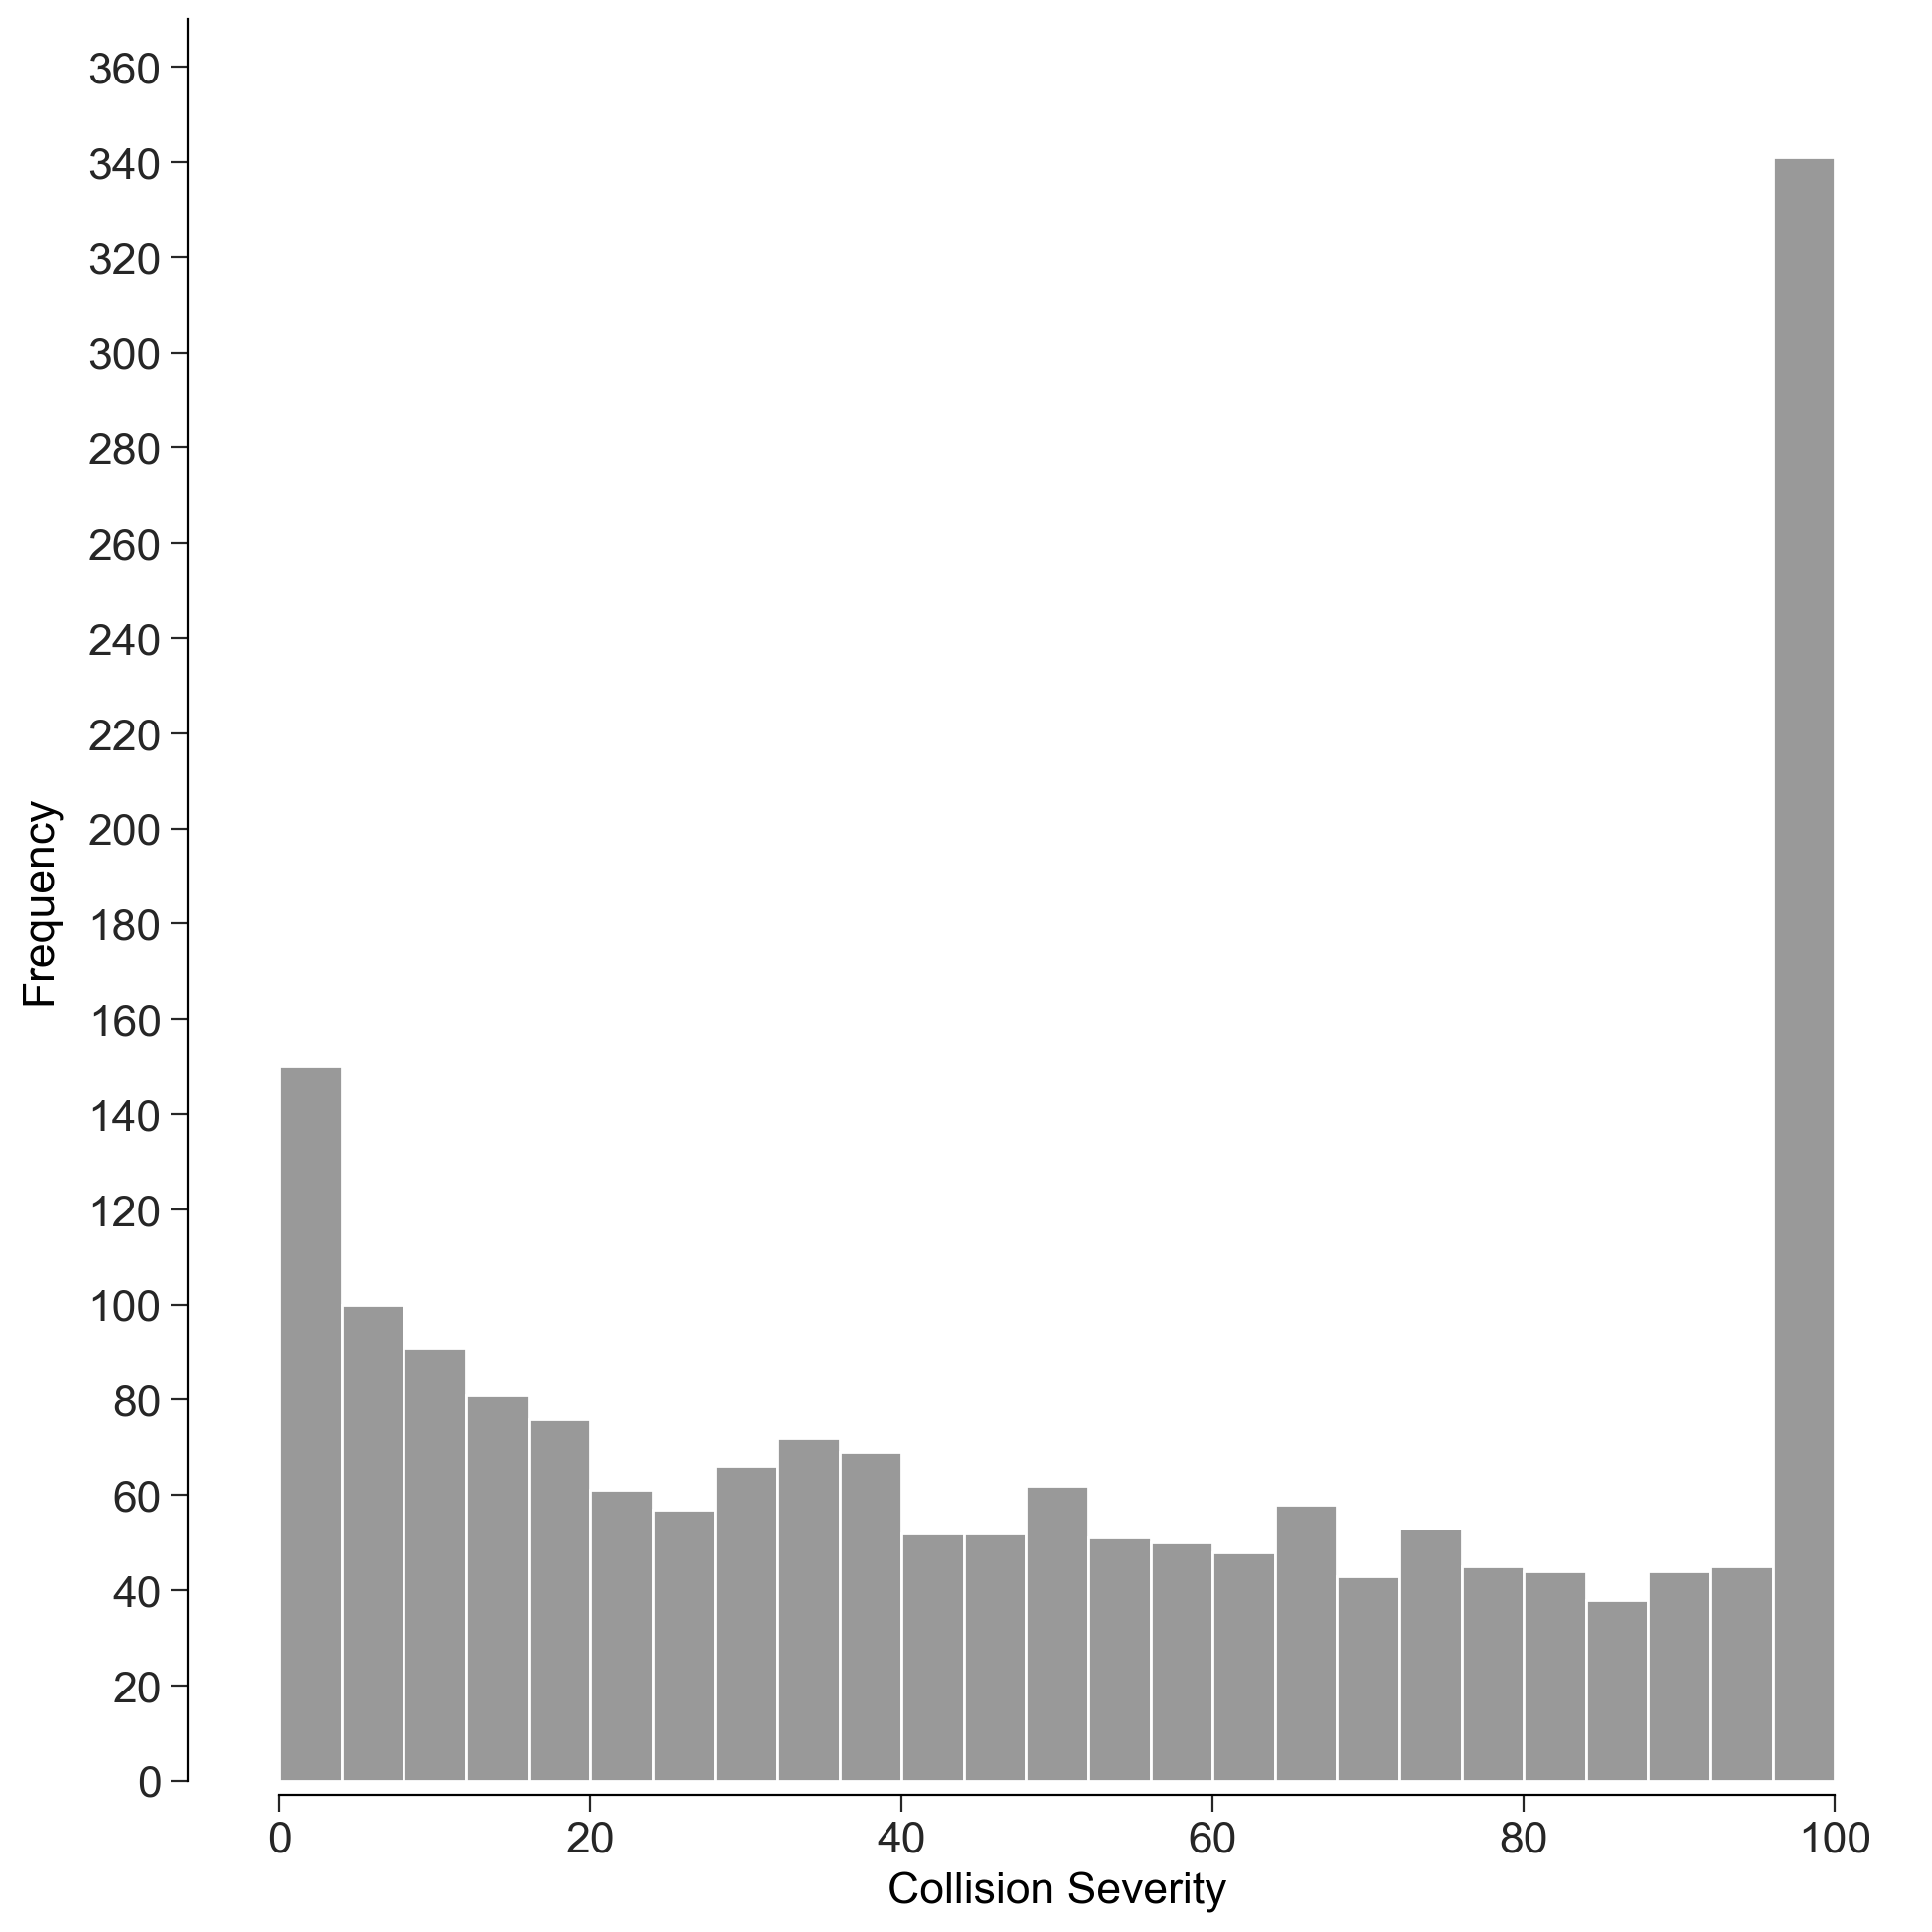
\includegraphics[height=.22\paperheight]{images/demonstration/rigid_failure_metric_histogram.png}
        \caption{Failure severity on flat rigid terrain for all obstacle configurations.}
        \label{fig:rigid_failure_metric_histogram}
    \end{subfigure}
    \caption{Additional metrics analyzing path length and collision directness.}
\end{figure}

%!TEX root = ../root.tex

\section{Conclusion and Future Work}
\label{sec:conclusions}
This contribution has two main themes. The first pertains a simulation platform, called Chrono, that supports AV off-road mobility studies. The second focuses on end-to-end learning as enabled by the Chrono environment, which anchors both the learning and testing phases. The end-to-end policy is used in flat and hilly landscapes, with deformable terrain that can be hard (silt-like) or soft (snow-like). We noted the following: policies learned on flat terrain are insufficient for navigating hilly scenarios; policies learned on rigid terrain transfer quite well to deformable terrain when the terrain is flat; the hillier the landscape, the harder it is to navigate it (Fig.\ref{fig:successRates}); the more obstacles are randomly placed on the course, the less likely it is for the policy to see the vehicle through; the control policy led to trip trajectories that came rather close to those associated with PSO, a third party trajectory planning tool (Fig.\ref{fig:pso_length_compare}); there is a sizable number of head-on collisions that point to room for improvement in the derived policy (Fig.\ref{fig:rigid_failure_metric_histogram}). Note that the testing conditions, in terms of average number of obstacles per unit area, were more harsh than the learning conditions.

Looking ahead, we plan to pursue several research thrusts and simulation platform development avenues. One direction is to investigate more complex control stacks that would combine the end-to-end with more traditional strategies such as model predictive control. The current work should be expanded to understand how tracked vehicles perform under similar conditions given that their traction and turning radius differ significantly from their wheel counterparts. Work is underway for faster SCM simulation that will allow straight training on deformable soil. Not analyzed in this contribution is the steering control input to the vehicle, which can often be noisy based on the output of the NN. Finally, we plan to investigate approaches that enhance the chance of simulation-derived policies transferring effectively to the real world.


%I reworked this section since it was a single sentence. I also dropped the reference to the noisy steering data since we never analyzed it. I think its good to mention it (I don't want to sweep anything under the rug), but I don't think we should put the results out there unless we can do it justice by analyzing and understanding it. - Asher

%more complex AV control stacks, that in addition to end-to-end policies bring into discussion model predictive control strategies; 

%the case of tracked vehicles, which are quite different than wheeled vehicles in that they can turn in place at zero translational velocity; 

%a faster SCM simulation strategy, which will allow training on deformable terrains; 

%how we can smooth out the steering wheel input produced by the policy -- it is far from what a human would do in that is aggressive in relation to left/right swings (plots not shown but available in supplemental material \cite{CoRLsupportData2020});

%and, approaches that improve the chances of simulation-derived policies to transfer to the real world.


%===============================================================================

% The maximum paper length is 8 pages excluding references and acknowledgements, and 10 pages including references and acknowledgements

\clearpage
% The acknowledgments are automatically included only in the final version of the paper.
\acknowledgments{This work was carried out in part with support from the Safety Research using Simulation (SAFER-SIM) program. SAFER-SIM is funded by a grant from the U.S. Department of Transportation’s University Transportation Centers Program (69A3551747131). The U.S. Government assumes no liability for the ideas expressed in this document or the use thereof.}

%===============================================================================

\bibliography{refs/newREFS,refs/refsSensors,refs/refsAutonomousVehicles,refs/refsChronoSpecific,refs/refsSBELspecific,refs/refsMBS,refs/refsTerramech,refs/refsRobotics,refs/refsStatsML}

\end{document}
